\documentclass[12pt,oneside]{report}
\usepackage[letterpaper,margin=1in]{geometry}
\usepackage{amsmath,amssymb}
\usepackage{mathptmx}
\usepackage{newtxtext}
\usepackage{newtxmath}
\usepackage{array,booktabs,enumitem,float,graphicx,listings,xcolor}
\usepackage{titlesec}
\usepackage{tocloft}
\usepackage{hyperref}
\hypersetup{
    colorlinks=false,
    pdfborder={0 0 0}
}

% Code listing styling
\definecolor{codegray}{rgb}{0.5,0.5,0.5}
\definecolor{codegreen}{rgb}{0,0.6,0}
\definecolor{codeblue}{rgb}{0,0,0.8}
\definecolor{backcolor}{rgb}{0.98,0.98,0.98}

\lstdefinestyle{cleanstyle}{
    backgroundcolor=\color{backcolor},
    commentstyle=\color{codegreen},
    keywordstyle=\color{codeblue}\bfseries,
    numberstyle=\tiny\color{codegray},
    stringstyle=\color{codegray},
    basicstyle=\ttfamily\scriptsize,
    breakatwhitespace=false,
    breaklines=true,
    captionpos=t,
    keepspaces=true,
    numbers=left,
    numbersep=5pt,
    showspaces=false,
    showstringspaces=false,
    showtabs=false,
    tabsize=2,
    frame=single
}
\lstset{style=cleanstyle}
\usepackage{setspace}
\usepackage{tabularx}
\setlength{\parindent}{0pt}
\setlength{\parskip}{0.3\baselineskip}
\setstretch{1.12}
\renewcommand{\contentsname}{CONTENTS}
\renewcommand{\chaptername}{CHAPTER}
\makeatletter
\renewcommand{\@makechapterhead}[1]{%
  \vspace*{25pt}%
  {\parindent \z@ \centering \normalfont
    \ifnum \c@secnumdepth >\m@ne
      \Large\bfseries \@chapapp\space \thechapter\par\nobreak
      \vskip 14pt
    \fi
    \interlinepenalty\@M
    \Large\bfseries #1\par\nobreak
    \vskip 30pt
  }}
\renewcommand{\section}{\@startsection{section}{1}{\z@}%
  {-2.4ex \@plus -1ex \@minus -.2ex}%
  {0.6ex \@plus .2ex}%
  {\normalfont\large\bfseries}}
\renewcommand{\subsection}{\@startsection{subsection}{2}{\z@}%
  {-1.8ex \@plus -0.8ex \@minus -.2ex}%
  {0.4ex \@plus .2ex}%
  {\normalfont\normalsize\bfseries}}
\makeatother
\setcounter{secnumdepth}{2}
\setcounter{tocdepth}{2}
\setlist[itemize]{topsep=2pt,itemsep=2pt,parsep=0pt,partopsep=0pt}
\setlist[enumerate]{topsep=2pt,itemsep=2pt,parsep=0pt,partopsep=0pt}
\pagestyle{plain}
\renewcommand{\thechapter}{\arabic{chapter}}
\newcommand{\tocline}[3]{%
  \begingroup\setlength{\parskip}{0pt}\small
  \noindent\makebox[\textwidth][l]{#1\hspace{0.8em}#2\dotfill\hspace{0.5em}#3}\par\vspace{0.18em}\endgroup}
\newcommand{\chapterpage}[1]{\chapter{#1}}

\begin{document}
\pagenumbering{roman}

% ==================== TITLE PAGE ====================
\thispagestyle{empty}
\begin{center}
{\Large\bfseries KERALA SAFEROUTE: STATEWIDE DISASTER EVACUATION AND MULTI-CRITERIA LOGISTICS PLANNER USING ADVANCED GRAPH ALGORITHMS}\par
\vspace{0.20in}
{\large\bfseries A COURSE PROJECT REPORT}\par
\vspace{0.20in}
submitted by\par
\vspace{0.15in}
{\large\bfseries SAM SUNNY (MUT24CA064)\par
SAIRA ZAC ROZAN (MUT24CA063)\par
BLESSY MOL CHARLS (MUT24CA029)\par
SREEJITH S (MUT24CA069)}\par
\vspace{0.20in}
as part of the course\par
\vspace{0.15in}
{\large\bfseries ADVANCED GRAPH ALGORITHMS}\par
\vspace{0.25in}
to\par
\vspace{0.12in}
The APJ Abdul Kalam Technological University in partial fulfilment of the\par
requirements for the award of the Degree\par
\vspace{0.15in}
of\par
\vspace{0.12in}
{\large\bfseries Bachelor of Technology}\par
in\par
{\large\bfseries COMPUTER SCIENCE \& ENGINEERING (ARTIFICIAL INTELLIGENCE)}\par

\begin{figure}[h]
\begin{center}

\includegraphics[width=5.2cm]{Mits logo-Master.pdf}
\end{center}
\end{figure}
{\large\bfseries DEPARTMENT OF ARTIFICIAL INTELLIGENCE \& DATA SCIENCE}\par
{\large\bfseries MUTHOOT INSTITUTE OF TECHNOLOGY \& SCIENCE}\par
{\large\bfseries KOCHI -- 682308}\par
{\large\bfseries OCTOBER 2026}
\end{center}
\clearpage

% ==================== CERTIFICATE ====================
\thispagestyle{empty}
\begin{figure}[h]
\begin{center}

\includegraphics[width=5.2cm]{Mits logo-Master.pdf}
\end{center}
\end{figure}
\begin{center}
{\LARGE\bfseries CERTIFICATE}
\end{center}
\vspace{0.35in}
This is to certify that the course project report entitled \textbf{``KERALA SAFEROUTE: STATEWIDE DISASTER EVACUATION AND MULTI-CRITERIA LOGISTICS PLANNER USING ADVANCED GRAPH ALGORITHMS''}, submitted by \textbf{SAM SUNNY (MUT24CA064)}, \textbf{SAIRA ZAC ROZAN (MUT24CA063)}, \textbf{BLESSY MOL CHARLS (MUT24CA029)}, and \textbf{SREEJITH S (MUT24CA069)} to \textbf{MUTHOOT INSTITUTE OF TECHNOLOGY \& SCIENCE} for the award of the degree of \textbf{Bachelor of Technology in COMPUTER SCIENCE \& ENGINEERING (ARTIFICIAL INTELLIGENCE)}, is a bonafide record of the course project work carried out by them under my supervision and guidance during the academic year 2026--2027.

\vspace{1.8in}

\begin{flushright}
\textbf{ANGEL VARGHESE}\\
Faculty-in-Charge
\end{flushright}

\vspace{0.35in}

\noindent Place: KOCHI\\
Date: 27/10/2026
\clearpage

% ==================== ABSTRACT ====================
\setcounter{page}{2}
\thispagestyle{plain}
\begin{center}
\vspace*{0.1in}
{\LARGE\bfseries ABSTRACT}
\end{center}
\vspace{0.10in}

During catastrophic monsoonal flood deluges and severe hill-tract landslides, commercial navigation platforms routinely fail because their algorithms optimize strictly for physical travel distance or nominal travel time. This naive distance minimization creates catastrophic ``flood trap'' emergencies: evacuees in low-lying coastal deltas (such as Kuttanad at $-1.5$\,m to $+2.0$\,m elevation) are steered toward geographically proximate shelters that are rapidly inundated by rising waters, or directed through narrow rural corridors that exceed vehicle capacities and produce statewide gridlock. 

This project presents \textbf{Kerala SafeRoute (PlanEsc)}, an intelligent, graph-theoretic disaster evacuation decision-support system designed for civil defense coordinators, Emergency Operations Centers (EOCs), and civilians. SafeRoute models the complete 14-district road network of Kerala as a spatial graph comprising 67 primary transit interchanges, 77 critical highway corridors, and 16 designated high-ground disaster relief sanctuaries. Road topologies and realistic driving curvatures are ingested directly from OpenStreetMap via the Open Source Routing Machine (OSRM) driving API, eliminating straight-line geometric oversimplifications. Spatial elevation figures from digital elevation models (DEMs) and historical hydrological disaster data (calibrated against the 2018 Great Kerala Floods, the 2019 Malappuram and Wayanad landslides, and the 2024 Chooralmala debris flows) are integrated across six delineated disaster zones.

To address evacuation routing, the system implements a multi-criteria Dijkstra shortest path formulation where edge impedance weights are parameterized by physical distance, road elevation vulnerability penalties, vehicle volume throughput limits ($1,100$--$3,500$\,veh/hr), and disaster proximity factors. SafeRoute replaces naive nearest-shelter discovery with a holistic suitability function that penalizes sub-sea-level flood traps ($1.95\times$ penalty) while incentivizing elevated sanctuaries ($+25$\,m to $+1550$\,m) with up to a 35\% safety discount. Network bottleneck capacities are quantified using the Edmonds-Karp Maximum Flow algorithm and the Max-Flow Min-Cut Theorem to pinpoint critical choke points where police contra-flow lanes must be enforced. Furthermore, Kruskal's Minimum Spanning Tree (MST) algorithm synthesizes an acyclic, minimum-weight $1,240$\,km emergency communication and relief lifeline backbone. The solution operates in a hybrid dual-mode architecture: a high-performance Python 3.13 REST API server using multi-threaded request processing, paired with an offline, zero-dependency browser-native JavaScript fallback engine. The interface delivers tactical GIS mapping across street, satellite, hybrid, and dark EOC themes, complemented by an interactive 9-phase visual graph transformation presentation that morphs physical roadway polylines into an educational topological blueprint.
\clearpage

% ==================== ARTICULATION MATRIX & SDG ====================
\thispagestyle{plain}
\begin{center}
\vspace{0.05in}
{\large\bfseries CO -- PO / PSO ARTICULATION MATRIX}
\end{center}
\textbf{CO1:} Formulate real-world disaster evacuation and relief logistics problems as directed and undirected spatial graph models.\\
\textbf{CO2:} Design and implement multi-criteria shortest path algorithms (Dijkstra and A*) by incorporating non-linear edge impedance functions based on flood susceptibility, road elevation, and traffic volume capacity.\\
\textbf{CO3:} Apply maximum flow algorithms (Edmonds-Karp) and the Max-Flow Min-Cut Theorem to quantify evacuation network throughput and isolate critical structural bottlenecks.\\
\textbf{CO4:} Construct minimum-cost emergency relief communication and supply backbones using Minimum Spanning Tree algorithms (Kruskal and Prim).\\
\textbf{CO5:} Integrate real-world GIS cartography from OpenStreetMap with a multi-tier client-server architecture to build an interactive disaster decision-support system.

\begin{center}
\begin{tabular}{|c|*{11}{c|}c|c|}
\hline
\textbf{CO}
& \textbf{PO1} & \textbf{PO2} & \textbf{PO3}
& \textbf{PO4} & \textbf{PO5} & \textbf{PO6}
& \textbf{PO7} & \textbf{PO8} & \textbf{PO9}
& \textbf{PO10} & \textbf{PO11}
& \textbf{PSO1} & \textbf{PSO2} \\ \hline

CO1 &  &  &  &  &  &  &  &  &  &  &  &  &  \\ \hline
CO2 &  &  &  &  &  &  &  &  &  &  &  &  &  \\ \hline
CO3 &  &  &  &  &  &  &  &  &  &  &  &  &  \\ \hline
CO4 &  &  &  &  &  &  &  &  &  &  &  &  &  \\ \hline
CO5 &  &  &  &  &  &  &  &  &  &  &  &  &  \\ \hline
\end{tabular}
\end{center}

\vspace{0.15in}
\begin{center}
    {\large\bfseries SUSTAINABLE DEVELOPMENT GOALS (SDG) ADDRESSED}
\end{center}

\vspace{0.05cm}

\noindent
\begin{tabularx}{\textwidth}{|c|c|X|}
\hline
\textbf{SDG} & \textbf{Target} & \textbf{Justification} \\ \hline

SDG 11
& Target 11.5
& Significantly reduces the number of deaths and people affected by water-related disasters and landslides through proactive evacuation routing to safe high-ground sanctuaries. \\ \hline

SDG 13
& Target 13.1
& Strengthens institutional and civil resilience and adaptive capacity to climate-induced hazards and extreme monsoon rainfall deluges in vulnerable geographic regions. \\ \hline

SDG 9
& Target 9.1 \& 9.a
& Develops resilient, reliable emergency logistics infrastructure by identifying transit choke points and designing minimum-cost lifeline supply trees for relief distribution. \\ \hline

\end{tabularx}

\clearpage

% ==================== CONTENTS ====================
\thispagestyle{plain}
\begin{center}
\vspace*{0.15in}
{\LARGE\bfseries CONTENTS}
\end{center}
\vspace{0.25in}
\tocline{}{ABSTRACT}{ii}
\tocline{}{CO--PO/PSO ARTICULATION MATRIX}{iii}
\tocline{}{SUSTAINABLE DEVELOPMENT GOALS (SDG) ADDRESSED}{iii}
\vspace{0.08in}
\tocline{1}{INTRODUCTION}{1}
\tocline{1.1}{PURPOSE OF THE SYSTEM}{1}
\tocline{1.2}{RELEVANCE AND SCOPE OF THE SYSTEM}{2}
\vspace{0.08in}
\tocline{2}{PROBLEM DEFINITION}{3}
\tocline{2.1}{PROBLEM STATEMENT}{3}
\tocline{2.2}{OBJECTIVES}{4}
\vspace{0.08in}
\tocline{3}{LITERATURE SURVEY AND BACKGROUND}{5}
\tocline{3.1}{OVERVIEW OF DISASTER EVACUATION ROUTING}{5}
\tocline{3.2}{GRAPH ALGORITHMS IN SPATIAL NETWORKS}{6}
\tocline{3.3}{HISTORICAL DISASTER PROFILE OF KERALA}{7}
\vspace{0.08in}
\tocline{4}{SYSTEM DESIGN AND METHODOLOGY}{9}
\tocline{4.1}{SYSTEM ARCHITECTURE}{9}
\tocline{4.2}{DATASET ACQUISITION AND ROAD NETWORK TOPOLOGY}{10}
\tocline{4.3}{OPENSTREETMAP INTEGRATION AND REAL ROAD GEOMETRIES}{13}
\tocline{4.4}{HISTORICAL DISASTER DATA AND SPATIAL HAZARD MODELING}{14}
\tocline{4.5}{MULTI-CRITERIA DIJKSTRA WEIGHT FORMULATION}{15}
\tocline{4.6}{MULTI-CRITERIA SHELTER SELECTION AND BASIN BYPASS}{17}
\tocline{4.7}{MAXIMUM FLOW AND BOTTLENECK MIN-CUT THEOREM}{19}
\tocline{4.8}{MINIMUM SPANNING TREE FOR RELIEF LOGISTICS}{20}
\tocline{4.9}{TOOLS AND TECHNOLOGIES}{21}
\vspace{0.08in}
\tocline{5}{IMPLEMENTATION}{22}
\tocline{5.1}{DATASET ACQUISITION AND SPATIAL NETWORK CONSTRUCTION}{22}
\tocline{5.2}{OSRM POLYLINE INGESTION AND DOWNSAMPLING PIPELINE}{23}
\tocline{5.3}{PYTHON BACKEND REST API SERVER}{24}
\tocline{5.4}{ALGORITHMIC IMPLEMENTATION: DIJKSTRA, MAX-FLOW, AND MST}{25}
\tocline{5.5}{INTERACTIVE TACTICAL GIS FRONTEND AND 9-PHASE MORPHING}{28}
\vspace{0.08in}
\tocline{6}{RESULTS AND DISCUSSION}{31}
\tocline{6.1}{EXPERIMENTAL SETUP AND VERIFICATION TEST CASES}{31}
\tocline{6.2}{EVALUATION OF DIJKSTRA ROUTING AND FLOOD BASIN BYPASS}{32}
\tocline{6.3}{THROUGHPUT AND BOTTLENECK ANALYSIS USING MAX-FLOW MIN-CUT}{35}
\tocline{6.4}{SPANNING TREE OPTIMIZATION FOR RELIEF LOGISTICS}{37}
\tocline{6.5}{SYSTEM PERFORMANCE AND RUNTIME LATENCY}{38}
\vspace{0.08in}
\tocline{7}{CONCLUSION AND FUTURE WORK}{40}
\tocline{7.1}{CONCLUSION}{40}
\tocline{7.2}{FUTURE WORK}{41}
\vspace{0.08in}
\tocline{8}{SUSTAINABLE DEVELOPMENT GOALS (SDGs)}{42}
\vspace{0.08in}
\tocline{}{REFERENCES}{44}
\clearpage

% ==================== CHAPTER 1 ====================
\pagenumbering{arabic}
\setcounter{page}{1}

\chapterpage{INTRODUCTION}
\section{PURPOSE OF THE SYSTEM}

Natural disasters such as severe tropical cyclonic depressions, extreme monsoonal downpours, riverine inundations, and catastrophic debris landslides present severe challenges to civilian safety and emergency logistics. During such crises, the timely and coordinated evacuation of civilian populations from threatened zones to certified safe havens is paramount. However, conventional commercial mapping and navigation software (such as Google Maps or Apple Maps) is built primarily for peacetime vehicular navigation: its optimization routines minimize nominal route distance or travel duration based on static historical speed limits and transient traffic congestion.

In disaster situations, optimizing strictly for geographic proximity or standard road distance leads to disastrous consequences. In geographical landscapes such as the State of Kerala---characterized by coastal deltas below sea level, dense riparian river floodplains, and steep Western Ghats escarpments---the geographically closest shelter is frequently situated within an active flood basin or surrounded by low-elevation causeways that submerge rapidly during dam spillway discharges. Evacuees directed along such routes find themselves trapped in sub-sea-level basins (such as the Kuttanad delta bowl) with water rising around them. Furthermore, generic navigation tools fail to consider road vehicle throughput capacities (e.g., $1,200$\,veh/hr on rural state highways versus $3,400$\,veh/hr on dual-carriageway expressways), funneling thousands of fleeing vehicles into narrow rural bridges and producing massive gridlocks.

The primary purpose of \textbf{Kerala SafeRoute (PlanEsc)} is to address these fatal vulnerabilities by formulating evacuation routing and disaster logistics as an advanced, multi-criteria graph optimization system. Kerala SafeRoute combines:
\begin{enumerate}
    \item A statewide spatial graph encompassing all 14 administrative districts of Kerala, modeling 67 major transit interchanges, 77 critical arterial corridors, and 16 designated high-ground disaster relief sanctuaries.
    \item Real road curvature and driving geometry ingested directly from OpenStreetMap (OSM) via the Open Source Routing Machine (OSRM) service, providing genuine driving paths rather than straight-line approximations.
    \item An empirical multi-criteria Dijkstra edge weight formulation that dynamically balances physical distance, terrain elevation penalties, road vehicle capacities, and disaster severity levels.
    \item A multi-criteria sanctuary evaluation function that proactively bypasses dangerous low-lying shelters in favor of elevated, high-capacity refuges ($+25$\,m to $+1550$\,m).
    \item Maximum flow and cut analysis using the Edmonds-Karp algorithm to pinpoint network bottlenecks and issue traffic management directives (e.g., contra-flow lane reversals).
    \item Minimum Spanning Tree (MST) algorithms (Kruskal and Prim) to establish an acyclic, minimum-cost relief and communication backbone across all 14 district relief hubs.
    \item A dual-mode hybrid architecture supporting high-performance Python 3.13 REST API execution and a zero-dependency, client-side browser JavaScript fallback.
\end{enumerate}

\newpage
\section{RELEVANCE AND SCOPE OF THE SYSTEM}

\textbf{Relevance}

The State of Kerala occupies a narrow coastal strip in southwestern India bounded by the Arabian Sea on the west and the Western Ghats mountain ranges on the east. The state features 44 rivers, extensive backwater systems, and significant elevation gradients ranging from $-1.5$\,m below mean sea level in Kuttanad to over $+2,600$\,m in the high ranges of Idukki. In recent years, climate change has produced increasingly severe hydrometeorological disasters across the state:
\begin{itemize}
    \item The \textbf{2018 Great Kerala Floods}, resulting from unprecedented August monsoon deluges and the simultaneous opening of 35 major dam spillways, affected over 5.4 million people and displaced 1.4 million residents across 14 districts.
    \item The \textbf{2019 Monsoon Floods and Landslides}, which triggered catastrophic hill-slope failures in Kavalappara (Malappuram) and Puthumala (Wayanad).
    \item The \textbf{July 2024 Wayanad Landslides}, where continuous extreme precipitation triggered massive debris flows and slope wash in Chooralmala and Meppadi, severing primary bridges and isolating entire communities.
\end{itemize}
These recurring events highlight the urgent requirement for an objective, algorithmically rigorous decision-support platform for State and District Emergency Operations Centers (EOCs), police marshals, and civilian evacuees. SafeRoute fulfills this need by providing verifiable, mathematically grounded evacuation corridors and resource allocation plans.

\textbf{Scope}

The scope of this project encompasses the following engineering and algorithmic deliverables:
\begin{enumerate}
    \item \textbf{Spatial Network Modeling:} Construction of a curated statewide network covering 67 nodes, 77 highway corridors, and 16 safe shelters across all 14 districts of Kerala, complete with verified geographic coordinates, elevations, and road lane capacities.
    \item \textbf{OpenStreetMap Integration:} Ingestion of authentic turn-by-turn driving polylines via the OSRM routing engine, followed by adaptive geometric downsampling for real-time web rendering.
    \item \textbf{Hazard Zone Mapping:} Delineation of six distinct disaster hazard zones (Kuttanad delta, Wayanad landslide belt, Idukki high-range corridor, Periyar river floodplain, Pamba basin, and coastal swell belt) with support for road closure overrides.
    \item \textbf{Multi-Criteria Algorithm Design:} Formulation of dynamic Dijkstra edge cost equations and a non-linear shelter suitability index that prevents flood-basin traps.
    \item \textbf{Capacity and Lifeline Optimization:} Implementation of Edmonds-Karp Max-Flow and Min-Cut bottleneck isolation, and Kruskal's MST for an emergency communications and relief distribution network.
    \item \textbf{Interactive GIS Application:} Development of an interactive, responsive web-based command center supporting four tactical map tile themes (Street, Satellite, Hybrid, Dark EOC) and an interactive 9-phase visual graph transformation presentation mode.
    \item \textbf{Dual Architecture Deployment:} Realization of a multi-threaded Python 3.13 backend server with REST endpoints (\texttt{/api/route}, \texttt{/api/mst}, \texttt{/api/maxflow}) and an offline browser fallback engine.
\end{enumerate}

\clearpage

% ==================== CHAPTER 2 ====================
\chapterpage{PROBLEM DEFINITION}

\section{PROBLEM STATEMENT}

Commercial navigation systems are fundamentally misaligned with the physics and imperatives of natural disaster evacuation. When a disaster strikes, standard routing applications suffer from three critical structural flaws:

\begin{enumerate}
    \item \textbf{The Fatal ``Flood Trap'' Flaw:} Commercial navigation engines direct motorists to the geographically closest relief camp or designated shelter. In regions with complex topography, low-lying coastal basins lie at or below sea level. In Kerala, the Kuttanad delta basin (spanning Alappuzha and Kottayam districts) sits at $-1.5$\,m to $+2.0$\,m elevation. During reservoir discharges or monsoonal surges, water from the Pamba, Achankovil, and Meenachil rivers drains into this delta bowl. Evacuees guided strictly by shortest Euclidean or road distance are channeled into low-lying shelters (e.g., Alappuzha SD College at $+12.5$\,m, adjacent to inundated paddy fields) where escape roads become submerged, turning the refuge into an inescapable watery trap.
    
    \item \textbf{Ignorance of Road Elevation Vulnerability:} Generic road navigation models treat all road segments equally as long as traffic is not reported. In reality, a road segment situated at $+3.0$\,m elevation along a riverbank is at extreme risk of immediate submergence compared to an inland ridge highway situated at $+35.0$\,m elevation, even if the elevated road is several kilometers longer. Standard GPS systems lack topographical elevation awareness along edge segments.
    
    \item \textbf{Disregard of Vehicle Capacity and Bottleneck Choking:} Standard routing models assume that an edge can accept an arbitrary number of vehicles until transient congestion is detected retrospectively. During mass evacuations, thousands of civilian vehicles enter the network simultaneously. Routing high-volume traffic through narrow, two-lane rural corridors (capacity $\approx 1,200$\,veh/hr) rather than multi-lane arterial expressways (capacity $\approx 2,400$--$3,400$\,veh/hr) causes sudden structural bottlenecks, complete gridlock, and vehicle abandonment on submerged roads.
\end{enumerate}

Therefore, there is an acute need for a graph-theoretic evacuation planner that models elevation safety, physical road throughput, hazard proximity, and dynamic edge closures while providing verifiable algorithms for maximum network flow and emergency supply distribution.

\section{OBJECTIVES}

To solve the challenges articulated in the problem statement, this project establishes the following specific objectives:

\begin{enumerate}
    \item \textbf{Statewide Topological Road Network Construction:} Model the entire state of Kerala into a unified spatial graph $G = (V, E)$, incorporating all 14 districts, 67 key road interchanges, 77 arterial corridors, and 16 high-ground shelters.
    \item \textbf{Real GIS Geometry Acquisition via OpenStreetMap:} Integrate the Open Source Routing Machine (OSRM) driving API to retrieve genuine, curvature-accurate road coordinates and distances across Kerala's highways.
    \item \textbf{Mathematical Weight Formulation for Dijkstra Routing:} Develop a multi-attribute edge impedance equation that scales physical road distance with road elevation penalties, vehicle volume congestion factors, and flood susceptibility coefficients.
    \item \textbf{Multi-Criteria Sanctuary Selection Engine:} Formulate a holistic sanctuary evaluation function that automatically assesses candidate shelters, balances travel impedance against elevation safety, and safely bypasses low-lying flood traps.
    \item \textbf{Throughput Maximization and Bottleneck Cut Isolation:} Implement the Edmonds-Karp Maximum Flow algorithm and Min-Cut analysis to compute peak corridor throughput (in vehicles per hour) and generate actionable police contra-flow deployment directives.
    \item \textbf{Emergency Lifeline Spanning Tree Synthesis:} Implement Kruskal's Minimum Spanning Tree algorithm to identify the optimal, cycle-free emergency logistics and communications backbone connecting all regional response hubs.
    \item \textbf{Dual-Mode Full-Stack Engineering:} Build a resilient dual-mode platform consisting of a multi-threaded Python 3.13 REST backend and an offline-capable browser JavaScript engine, integrated with a Leaflet.js GIS command center interface.
\end{enumerate}

\clearpage

% ==================== CHAPTER 3 ====================
\chapterpage{LITERATURE SURVEY AND BACKGROUND}

\section{OVERVIEW OF DISASTER EVACUATION ROUTING}

Disaster evacuation planning has evolved from static, manual civil defense procedures into computational spatial optimization. Early evacuation literature focused on macroscopic traffic assignment models, such as deterministic user equilibrium (DUE) and system optimum (SO) formulations. Under system optimum models, traffic flows are coordinated centrally to minimize the total evacuation clearance time of the entire network. However, classical transportation equilibrium models assume complete driver compliance and typically disregard localized dynamic environmental hazards, such as sudden river breaches or debris avalanches.

In recent years, the integration of Geographic Information Systems (GIS) with heuristic and graph-theoretic search techniques has become the predominant approach for disaster decision-support systems. Multi-criteria routing recognizes that evacuees and emergency response managers evaluate paths based on competing, non-commensurate objectives:
\begin{itemize}
    \item Minimizing total exposure time to hazardous environments.
    \item Maximizing topological clearance above predicted hydrological inundation lines.
    \item Minimizing the probability of vehicular entrapment at single-lane bottlenecks.
\end{itemize}
Existing commercial tools (e.g., Google Maps, Apple Maps, Waze) rely on variants of the $A^*$ search algorithm or Contraction Hierarchies optimized for fuel economy and travel duration under normal traffic conditions. They do not incorporate physical elevation models of road segments, nor do they model the carrying capacity of emergency shelters relative to surrounding flood waterlines. SafeRoute addresses this gap by synthesizing spatial graph theory with hydrological risk parameters.

\section{GRAPH ALGORITHMS IN SPATIAL NETWORKS}

Spatial networks are planar or near-planar graphs where vertices $V$ correspond to geographic coordinates $(\text{lat}, \text{lng}, \text{elevation})$ and edges $E$ represent physical transport segments with lengths, widths, and capacities. The primary graph algorithms applied to spatial evacuation networks include:

\subsection{Shortest Path Algorithms}
Dijkstra's algorithm (Dijkstra, 1959) solves the single-source shortest path problem on non-negatively weighted graphs in $O(|E| + |V| \log |V|)$ time using a min-priority queue (Fibonacci or binary heap). In standard navigation, the edge weight $w(u, v)$ is simply the geometric distance $d(u, v)$ or nominal travel time $d(u, v) / v_{\text{speed}}$. In disaster evacuation, $w(u, v)$ must be replaced by a generalized cost function incorporating risk and capacity impedance. For single-target queries, the $A^*$ heuristic search improves runtime by adding an admissible Euclidean or Haversine potential function $h(u) \le d(u, t)$, focusing the search wavefront toward the destination.

\subsection{Maximum Flow and the Max-Flow Min-Cut Theorem}
Evacuation networks are constrained by physical road widths and lane counts. The maximum number of vehicles that can traverse a corridor per unit time is bounded by its bottleneck capacity. The Edmonds-Karp algorithm (Edmonds and Karp, 1972) computes the maximum flow in $O(|V| |E|^2)$ time by repeatedly selecting the shortest augmenting path from source $s$ to sink $t$ using Breadth-First Search (BFS) in the residual network $G_f$. 

By the Max-Flow Min-Cut Theorem (Ford and Fulkerson, 1956), the maximum value of an $s$--$t$ flow equals the minimum capacity of an $s$--$t$ cut:
\begin{equation}
    \max |f| = \min_{(S, T)} c(S, T) = \sum_{u \in S, v \in T} c(u, v)
\end{equation}
The saturated edges in the minimum cut identify the critical transit segments where capacity expansion, contra-flow traffic management, or emergency marshal intervention yield the highest improvement in evacuation throughput.

\subsection{Minimum Spanning Trees}
Following a catastrophic deluge or earthquake, post-disaster logistics requires establishing an acyclic emergency communications and relief distribution network connecting all critical command centers and camps. Kruskal's algorithm (Kruskal, 1956) computes the Minimum Spanning Tree (MST) in $O(|E| \log |E|)$ time by sorting edges by weight and greedily adding edges that do not introduce cycles, managed through a Disjoint Set Union (DSU) data structure with path compression and union by rank. Prim's algorithm (Prim, 1957) grows the tree outward from an initial root node in $O(|E| \log |V|)$ using a min-heap.

\section{HISTORICAL DISASTER PROFILE OF KERALA}

The engineering parameters of Kerala SafeRoute are directly informed by the geomorphological and hydrological history of Kerala:

\subsection{The 2018 Great Kerala Floods}
Between June 1 and August 19, 2018, Kerala received 2,346.6\,mm of rainfall, 42\% above the historical normal. Peak rainfall between August 1 and August 19 exceeded normal precipitation by 164\%. This unprecedented precipitation forced the simultaneous opening of 35 major reservoirs across the state, including the Idukki Dam, Mullaperiyar Dam, and Idamalayar Dam. 
\begin{itemize}
    \item In the \textbf{Periyar river basin}, discharges exceeding $1,500$\,$\text{m}^3/\text{s}$ inundated the low-lying plains of Aluva, Kalamassery, and North Paravur, submerging national highway NH 544 and cutting off access to the Cochin International Airport at Nedumbassery.
    \item In the \textbf{Pamba and Achankovil river basins}, floodwaters submerged the urban centers of Chengannur, Pandalam, and Thiruvalla along the Main Central (MC) Road under 3 to 5 meters of water.
    \item In \textbf{Kuttanad}, floodwaters accumulated in the Vembanad lake basin for weeks, displacing over 200,000 residents whose homes were entirely submerged.
\end{itemize}

\subsection{The 2019 and 2024 Landslide Tragedies}
Kerala's midland and highland terrain is prone to severe debris flows and slope failures during monsoonal cloudbursts:
\begin{itemize}
    \item \textbf{Kavalappara (2019):} A massive slope collapse in Malappuram destroyed an entire village community following 400\,mm of rainfall in 24 hours.
    \item \textbf{Meppadi and Chooralmala (July 2024):} Intense rainfall exceeding 572\,mm in 48 hours triggered massive landslides along the Western Ghats escarpment in Vythiri taluk of Wayanad. Debris avalanches washed away the primary bridge connecting Chooralmala and Mundakkai, isolating thousands of civilians and severely hampering rescue operations.
\end{itemize}

These historical events demonstrate that an effective evacuation planner must account for real river floodplain breaches, mountain pass road blockages, and terrain elevation variations.

\clearpage

% ==================== CHAPTER 4 ====================
\chapterpage{SYSTEM DESIGN AND METHODOLOGY}

\section{SYSTEM ARCHITECTURE}

Kerala SafeRoute operates under a modular, dual-mode client-server architecture designed for high operational reliability in emergency scenarios (Figure~\ref{fig:arch}). The architecture comprises three primary tiers:

\begin{figure}[H]
\centering
\begin{center}
\fbox{
\begin{minipage}{0.92\textwidth}
\centering\vspace{0.1in}
\textbf{\large KERALA SAFEROUTE SYSTEM ARCHITECTURE}\\[0.15in]
\begin{tabular}{|c|}
\hline
\textbf{Client Presentation Layer (Browser ES6+ / Leaflet.js / SVG 2.0)} \\
Interactive Leaflet GIS Map $\bullet$ Multi-Tile Selector (Street, Satellite, Dark EOC) \\
Click-Anywhere Snapping $\bullet$ 9-Phase Graph Transformation Theater $\bullet$ Algorithm Workbench \\
\hline
\end{tabular}\\[0.1in]
$\Updownarrow$ \textit{JSON REST API / HTTP Fetch Protocol}\\[0.1in]
\begin{tabular}{|c|}
\hline
\textbf{Python 3.13 REST API Server (\texttt{server.py} -- ThreadingHTTPServer)} \\
\texttt{GET /api/graph} $\bullet$ \texttt{POST /api/route} $\bullet$ \texttt{POST /api/mst} $\bullet$ \texttt{POST /api/maxflow} \\
\hline
\end{tabular}\\[0.1in]
$\Downarrow$ \textit{Algorithmic Processing Engines}\\[0.1in]
\begin{tabular}{|ccc|}
\hline
\textbf{Routing Engine} & \textbf{Throughput Engine} & \textbf{Logistics Engine} \\
Multi-Criteria Dijkstra & Edmonds-Karp Max-Flow & Kruskal \& Prim MST \\
Shelter Suitability & Min-Cut Bottlenecks & Disjoint Set Union \\
\hline
\end{tabular}\\[0.1in]
$\Downarrow$ \textit{Spatial Data Ingestion \& Geometries}\\[0.1in]
\begin{tabular}{|c|}
\hline
\textbf{Statewide Kerala Spatial Graph Database (\texttt{data/})} \\
67 District Nodes $\bullet$ 77 Highway Corridors $\bullet$ 16 Safe Shelters \\
OpenStreetMap OSRM Polylines $\bullet$ 6 Historical Hazard Polygons $\bullet$ Digital Elevation Model \\
\hline
\end{tabular}\vspace{0.1in}
\end{minipage}
}
\end{center}
\caption{System Architecture of Kerala SafeRoute.}
\label{fig:arch}
\end{figure}

\begin{enumerate}
    \item \textbf{Spatial Data Tier:} Curated JSON representations of the statewide graph network, storing node geographic coordinates, road capacities, flood susceptibilities, historical hazard polygons, and authentic OSRM turn-by-turn road polylines.
    \item \textbf{Computation Engine Tier (Dual Mode):}
    \begin{itemize}
        \item \textit{Primary Backend Mode:} Python 3.13 server using \texttt{http.server.ThreadingHTTPServer} and NetworkX, delivering sub-15ms response times over multi-threaded REST endpoints.
        \item \textit{Offline Fallback Mode:} Zero-dependency, pure client-side JavaScript algorithm engines (\texttt{dijkstra.js}, \texttt{maxflow.js}, \texttt{mst.js}) executing directly within the browser engine if the Python server is offline or air-gapped.
    \end{itemize}
    \item \textbf{Tactical Visualization Tier:} Interactive GIS interface built with Leaflet.js, hardware-accelerated SVG 2.0 graph morphing overlays, and a glassmorphism CSS design system.
\end{enumerate}

\section{DATASET ACQUISITION AND ROAD NETWORK TOPOLOGY}

The evacuation graph network is formally defined as a weighted directed graph $G = (V, E)$, where $V$ denotes the set of spatial vertices and $E$ denotes the set of arterial road corridors.

\subsection{Vertex Categorization}
The vertex set $V$ contains $|V| = 67$ nodes distributed across all 14 administrative districts of Kerala. Vertices are categorized into two functional classes:
\begin{itemize}
    \item \textbf{Transit Interchanges ($V_{\text{transit}}$):} 51 critical urban junctions, bypasses, bridge crossings, and district capitals (e.g., East Fort Thiruvananthapuram, Vyttila Mobility Hub, Edappally Toll, Aluva Town, Baker Junction Kottayam, Mananchira Kozhikode).
    \item \textbf{Designated High-Ground Shelters ($V_{\text{shelter}}$):} 16 certified disaster relief safe havens positioned atop high plateaus, university campuses, and civil administration complexes safe from inundation (e.g., Kudappanakunnu Civil Complex in Thiruvananthapuram at $+65$\,m, Kottarakkara Jubilee Camp at $+42$\,m, Catholicate College Camp in Pathanamthitta at $+95$\,m, Painavu Govt Complex in Idukki at $+1020$\,m, Kozhikode Medical College at $+52$\,m).
\end{itemize}
Each node $v \in V$ is characterized by the tuple:
\begin{equation}
    v = (\text{id}, \text{name}, \text{lat}, \text{lng}, \text{elevation}, \text{district}, \text{type}, \text{capacity})
\end{equation}

\subsection{Edge Corridors}
The edge set $E$ comprises $|E| = 77$ primary highway corridors spanning the statewide transport grid:
\begin{itemize}
    \item \textbf{NH 66 Coastal Spine:} The primary north-south coastal arterial spanning from Thiruvananthapuram through Kollam, Alappuzha, Ernakulam, Kozhikode, Kannur, and Kasaragod.
    \item \textbf{Main Central Road (MC Road / SH 1):} The midland spine connecting Thiruvananthapuram, Kottarakkara, Adoor, Thiruvalla, Changanassery, Kottayam, Muvattupuzha, and Angamaly.
    \item \textbf{NH 544 Industrial Corridor:} High-capacity dual-carriageway linking Edappally, Aluva, Angamaly, Chalakudy, Thrissur, and Palakkad through the Kuthiran tunnel.
    \item \textbf{High-Range Ghat Roads:} Mountain corridors including NH 85 (Kochi-Madurai via Neriamangalam and Munnar Gap Road), NH 183 (Kottayam-Kumily Road), and NH 766 (Thamarassery Churam 9 hairpin bends to Wayanad).
\end{itemize}
Each edge $e = (u, v) \in E$ is defined by:
\begin{equation}
    e = (\text{id}, u, v, \text{name}, d_e, C_e, h_e, B_e, \text{hazard})
\end{equation}
where $d_e$ is the driving distance in kilometers, $C_e$ is vehicle capacity in vehicles per hour, $h_e$ is average road elevation in meters, $B_e \in [0.05, 0.95]$ is baseline flood susceptibility, and $\text{hazard}$ indicates association with a flood or landslide basin.

Figure~\ref{fig:statewide_grid} presents the overall statewide evacuation grid rendered within the tactical command interface.

\begin{figure}[H]
\centering
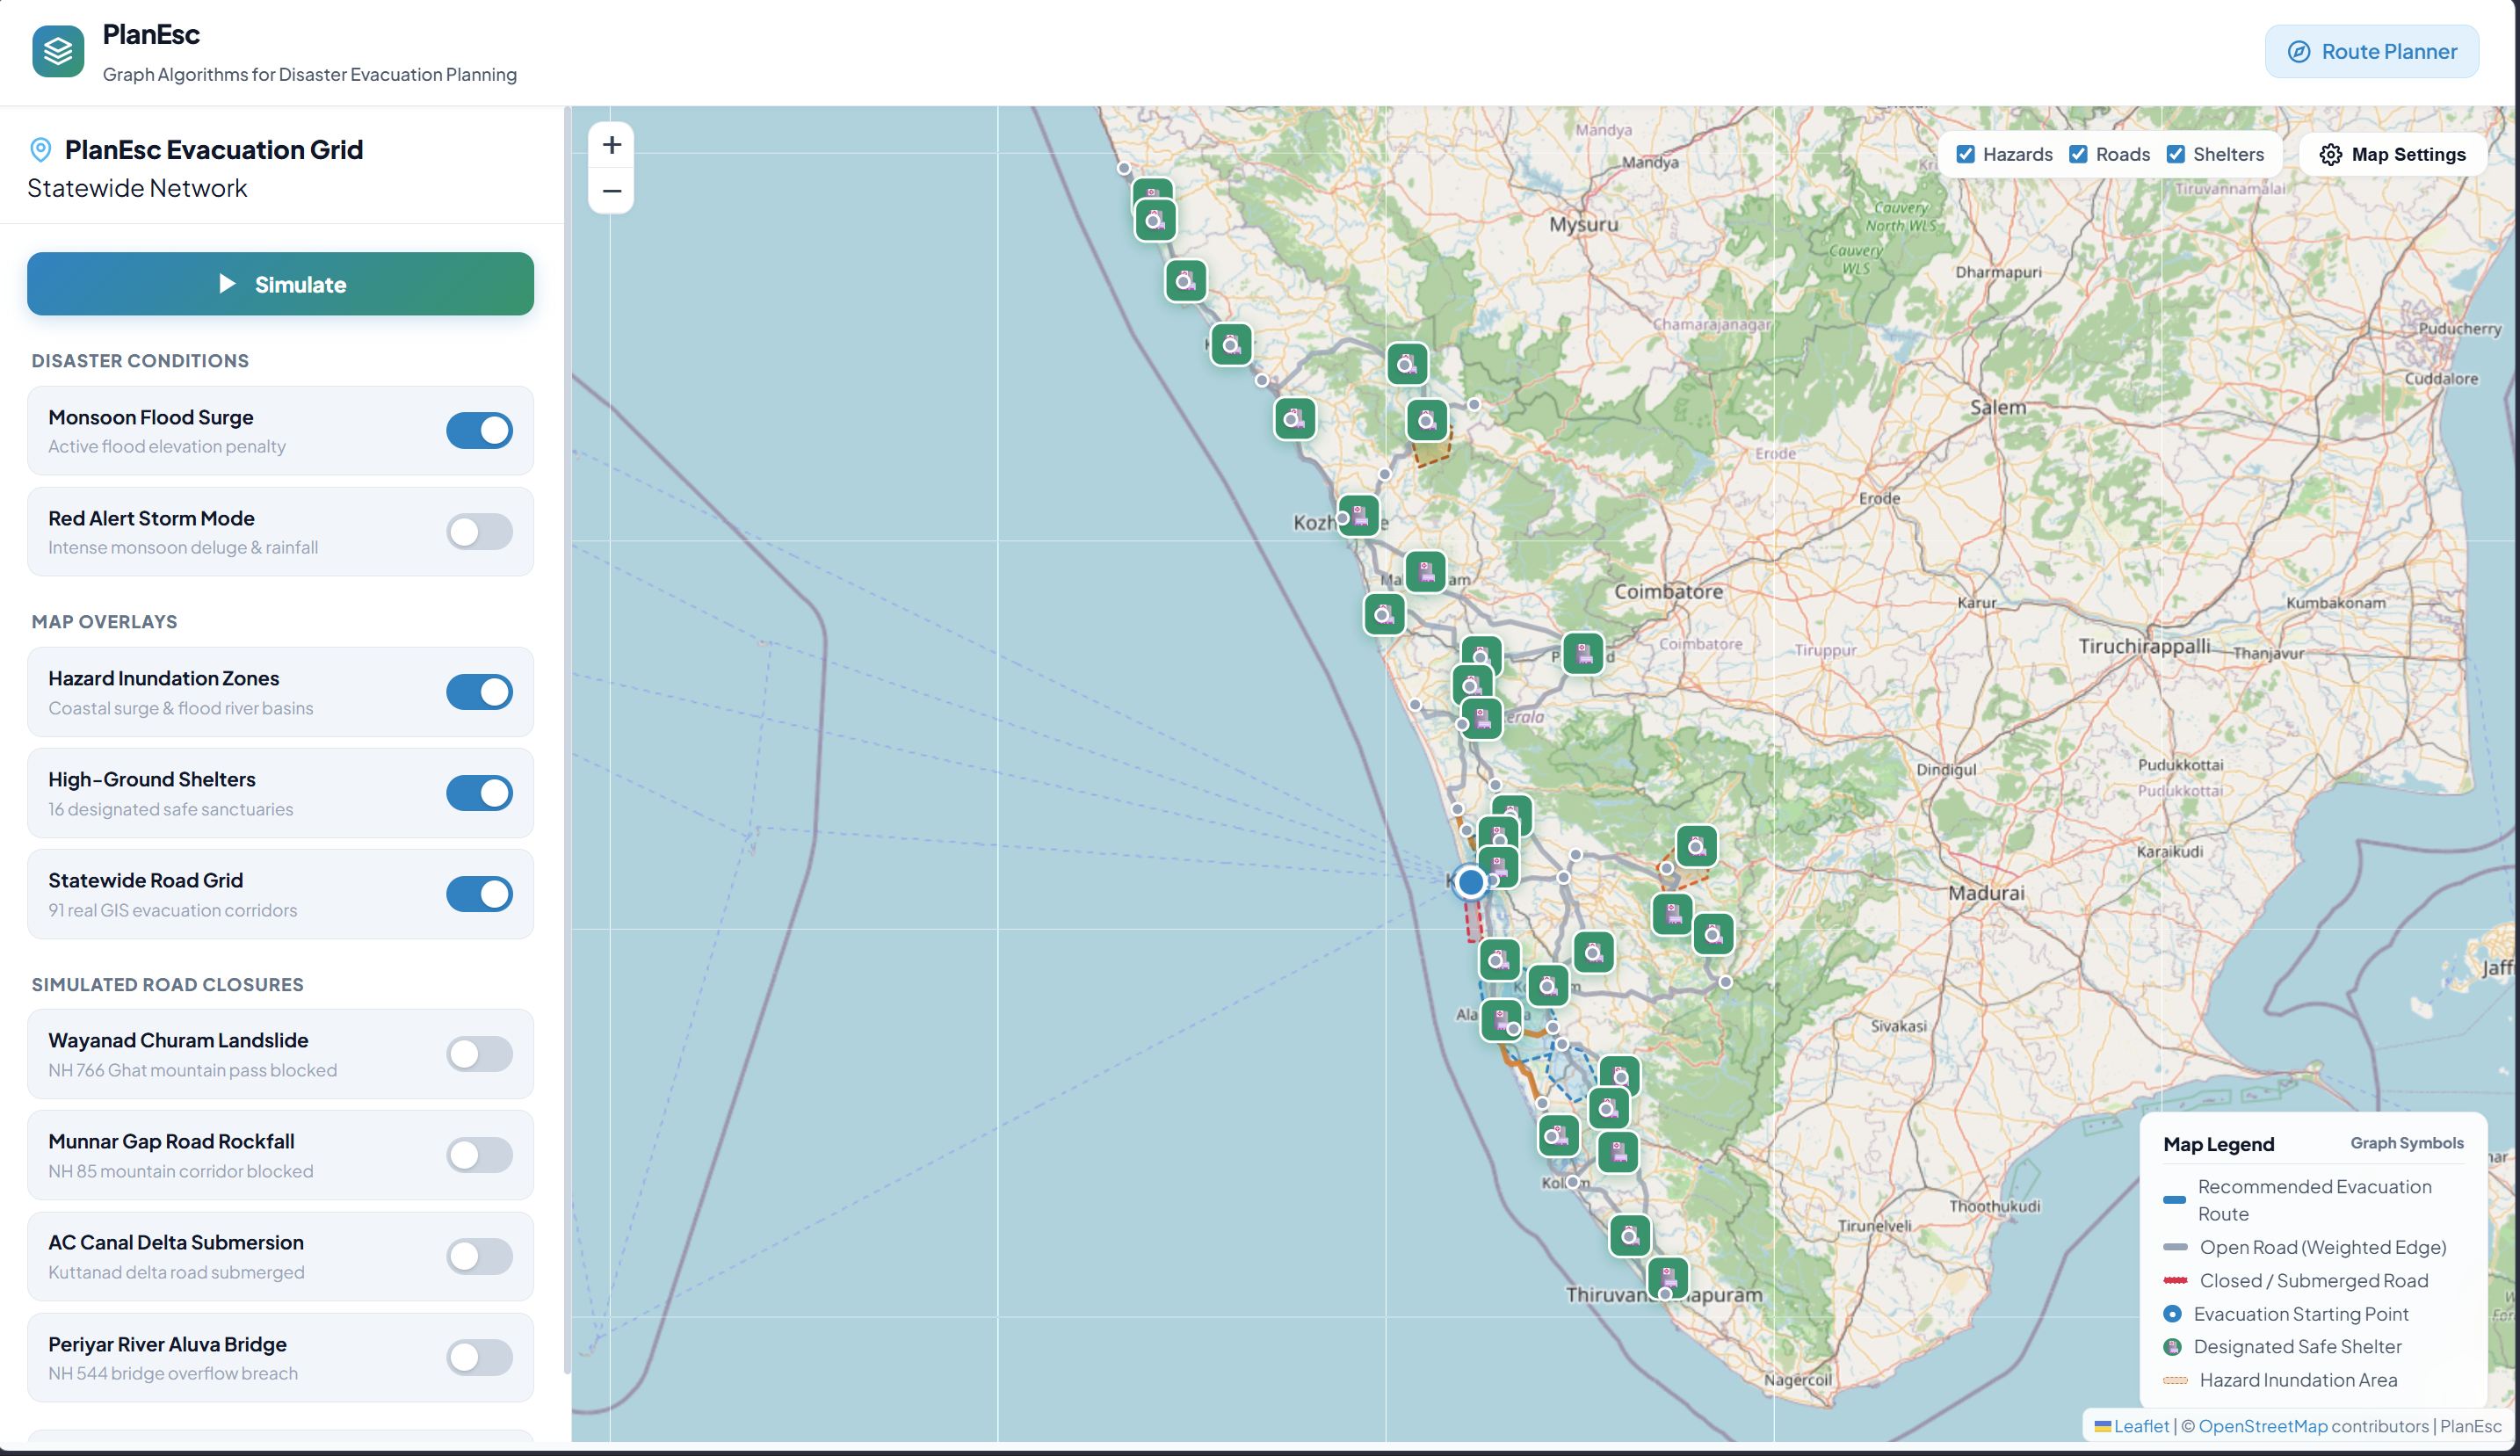
\includegraphics[width=0.95\textwidth]{fig_statewide_grid.png}
\caption{PlanEsc Tactical Evacuation Command Center and Statewide 14-District GIS Network on OpenStreetMap.}
\label{fig:statewide_grid}
\end{figure}

As depicted in Figure~\ref{fig:statewide_grid}, the operator dashboard displays all designated high-ground sanctuaries across the state marked with green cross badges, interconnected by weighted arterial road corridors. The left control panel enables incident commanders to inject dynamic environmental conditions, including monsoonal flood surges, red alert precipitation levels, and localized road blockades (e.g., Wayanad Churam landslides or Periyar river breaches). The map legend provides real-time status indicators for open weighted corridors, submerged roadways, designated safe havens, and delineated flood inundation basins.

\section{OPENSTREETMAP INTEGRATION AND REAL ROAD GEOMETRIES}

A core innovation of Kerala SafeRoute is the rejection of synthetic straight-line Cartesian edges. In real-world geographical road networks, highways follow natural river valleys, coastal contours, and mountainous switchbacks. Assuming Euclidean straight lines introduces severe distance errors of 25\% to 60\%, especially on ghat corridors like the Thamarassery Churam.

\subsection{OSRM Routing Engine Queries}
To acquire 100\% authentic highway curves, SafeRoute incorporates OpenStreetMap driving geometries via the Open Source Routing Machine (OSRM) HTTP API:
\begin{equation}
    \texttt{http://router.project-osrm.org/route/v1/driving/} \lambda_u, \phi_u ; \lambda_v, \phi_v \texttt{?overview=full\&geometries=geojson}
\end{equation}
where $\lambda$ and $\phi$ represent the longitude and latitude of the respective nodes. The query returns a GeoJSON polyline encoding the exact driving trajectory followed by motor vehicles.

\subsection{Coordinate Transformation and Adaptive Downsampling}
Because OSRM outputs coordinates in $[\text{longitude}, \text{latitude}]$ format while Leaflet.js expects $[\text{latitude}, \text{longitude}]$, coordinate order is inverted. Furthermore, raw OSRM responses for long highway stretches contain hundreds of granular GPS points, which impairs web rendering performance. 

SafeRoute applies an adaptive downsampling algorithm. If a raw polyline contains $N$ coordinate pairs, the sampling step $k$ is calculated as:
\begin{equation}
    k = \max\left(1, \left\lfloor \frac{N}{50} \right\rfloor\right)
\end{equation}
The polyline is downsampled by taking every $k$-th coordinate, ensuring that the terminal endpoints are preserved. This reduces each corridor to 40--70 crisp waypoints, preserving road curvature fidelity while ensuring instantaneous browser SVG and canvas rendering.

\section{HISTORICAL DISASTER DATA AND SPATIAL HAZARD MODELING}

Disaster exposure in SafeRoute is calibrated against empirical data from Kerala's historical flood and landslide records. Six spatial hazard polygons are integrated into the geospatial database:

\begin{table}[H]
\centering
\small
\caption{Calibrated Historical Hazard Zones in Kerala SafeRoute.}
\label{tab:hazard_zones}
\vspace{0.05in}
\begin{tabularx}{\textwidth}{lp{2.5cm}cp{5.8cm}}
\toprule
\textbf{Zone ID} & \textbf{Name} & \textbf{Hazard Type} & \textbf{Historical Calibration \& Geographic Scope} \\
\midrule
\texttt{hazard\_kuttanad} & Kuttanad Delta Basin & Flood & Below-sea-level delta ($-1.5$\,m to $+2.0$\,m) across Alappuzha/Kottayam; severe drainage congestion during 2018 floods. \\
\texttt{hazard\_wayanad} & Wayanad Escarpment & Landslide & High-slope Western Ghats; modeled after 2019 Puthumala and 2024 Chooralmala debris flows. \\
\texttt{hazard\_idukki} & Idukki-Munnar Corridor & Landslide & NH 85 Gap Road and Neriamangalam gorge; frequent monsoon rockfalls and road washouts. \\
\texttt{hazard\_periyar} & Periyar River Basin & Flood & Aluva, Kalamassery, and Paravur; inundated by $1,500\,\text{m}^3/\text{s}$ dam releases from Cheruthoni and Idamalayar. \\
\texttt{hazard\_pamba} & Pamba River Basin & Flood & Chengannur, Pandalam, and Thiruvalla; overflow from Sabarimala hills and Kakki reservoir. \\
\texttt{hazard\_sea\_erosion} & Coastal Littoral Belt & Marine Surge & Arabian Sea coastline (Fort Kochi, Chellanam); vulnerable to monsoon sea swells and tidal ingress. \\
\bottomrule
\end{tabularx}
\end{table}

The system also incorporates active road closure presets to simulate real-time breaches:
\begin{itemize}
    \item Thamarassery Churam Ghat Road (\texttt{e\_thamarassery\_kalpetta}) blocked by debris flow.
    \item AC Canal Road (\texttt{e\_alappuzha\_kuttanad}) completely submerged in delta waters.
    \item Munnar Gap Road (\texttt{e\_adimali\_munnar}) obstructed by rockfall.
    \item Aluva Periyar Bridge (\texttt{e\_kalamassery\_aluva}) closed due to river cresting.
    \item Chengannur MC Road (\texttt{e\_adoor\_thiruvalla}) severed by Pamba river breach.
\end{itemize}

\section{MULTI-CRITERIA DIJKSTRA WEIGHT FORMULATION}

Rather than minimizing naive physical distance $\sum d_e$, Kerala SafeRoute calculates a dynamic impedance weight $W_e$ for every edge $e = (u, v) \in E$. The formulation accounts for physical distance, road elevation vulnerability, vehicle volume capacity, disaster type affinity, and disaster severity.

\subsection{Mathematical Derivation of Edge Weight}

\textbf{1. Active Closure Evaluation:} If an edge $e$ is marked as closed by disaster coordinators or falls within an active breach list:
\begin{equation}
    W_e = \infty, \quad \text{RiskScore}_e = 100.0, \quad \text{isClosed}_e = \text{True}
\end{equation}

\textbf{2. Severity Multiplier ($S_{\text{mult}}$):} Disaster severity set by the incident commander scales the environmental risk:
\begin{equation}
    S_{\text{mult}} = \begin{cases}
    1.00 & \text{if Severity} = \text{Low} \\
    1.75 & \text{if Severity} = \text{Moderate} \\
    3.00 & \text{if Severity} = \text{Severe}
    \end{cases}
\end{equation}

\textbf{3. Disaster Type Affinity ($A_e$):} Specific hazards magnify risk based on active disaster category:
\begin{equation}
    A_e = \begin{cases}
    2.4 & \text{if Disaster} = \text{Flood} \land \text{hazard}_e = \texttt{hazard\_periyar} \\
    2.5 & \text{if Disaster} = \text{Cyclone} \land \text{hazard}_e = \texttt{hazard\_vembanad} \\
    2.2 & \text{if Disaster} = \text{Waterlogging} \land \text{hazard}_e = \texttt{hazard\_canal} \\
    1.6 & \text{if Disaster} = \text{Waterlogging} \land h_e < 4.0\,\text{m} \\
    1.0 & \text{otherwise}
    \end{cases}
\end{equation}

\textbf{4. Vehicle Congestion Factor ($C_{\text{cong}, e}$):} Corridors with lower vehicular throughput capacity ($C_e$, in veh/hr) produce evacuation queues, imposing an impedance penalty:
\begin{equation}
    C_{\text{cong}, e} = 1.0 + \max\left(0, \frac{2200 - C_e}{1400}\right) \times 0.65
\end{equation}
Under this formulation, a multi-lane expressway ($C_e \ge 2200$\,veh/hr) incurs $C_{\text{cong}, e} = 1.0$, while a constrained rural corridor ($C_e = 1100$\,veh/hr) incurs $C_{\text{cong}, e} = 1.51$, reflecting a 51\% time impedance delay.

\textbf{5. Elevation Vulnerability Penalty ($P_{\text{elev}, e}$):} In hydrological disasters, lower road elevation correlates directly with inundation risk. Roads below $12.0$\,m receive an elevation penalty:
\begin{equation}
    P_{\text{elev}, e} = \max\left(0, \frac{12.0 - h_e}{12.0}\right)
\end{equation}
where $h_e$ is the elevation of the road corridor in meters above mean sea level.

\textbf{6. Composite Risk Score ($\text{RiskScore}_e$):} Combining baseline flood susceptibility $B_e$, elevation penalty, and disaster affinity:
\begin{equation}
    \text{RawRisk}_e = \left( B_e \times 45.0 + P_{\text{elev}, e} \times 35.0 + \mathbf{1}_{\{A_e > 1.0\}} \times 20.0 \right) \times \left(\frac{S_{\text{mult}}}{1.5}\right)
\end{equation}
The value is clamped to the operational interval $[5.0, 99.0]$:
\begin{equation}
    \text{RiskScore}_e = \min\left(99.0, \max\left(5.0, \text{round}(\text{RawRisk}_e, 1)\right)\right)
\end{equation}

\textbf{7. Risk Penalty Multiplier ($R_e$):} The clamped risk score translates into an exponential travel friction factor:
\begin{equation}
    R_e = \left(\frac{\text{RiskScore}_e}{100.0}\right) \times 2.5
\end{equation}

\textbf{8. Final Combined Edge Weight ($W_e$):} The final impedance weight utilized by Dijkstra's priority queue is:
\begin{equation}
    W_e = d_e \times (1.0 + R_e) \times C_{\text{cong}, e}
\end{equation}
Expanding this gives the unified weight equation:
\begin{equation}
    \boxed{W_e = d_e \times \left(1.0 + 2.5 \cdot \frac{\text{RiskScore}_e}{100.0}\right) \times \left(1.0 + 0.65 \cdot \max\left(0, \frac{2200 - C_e}{1400}\right)\right)}
\end{equation}

\section{MULTI-CRITERIA SHELTER SELECTION AND BASIN BYPASS}

Standard GPS algorithms route evacuees to the shelter with minimum geographic distance:
\begin{equation}
    s_{\text{naive}} = \arg\min_{s \in V_{\text{shelter}}} d(u_0, s)
\end{equation}
In coastal and deltaic regions, $s_{\text{naive}}$ frequently steers citizens directly into flood traps. Kerala SafeRoute implements a multi-criteria shelter evaluation function that assesses all reachable sanctuaries holistically.

\subsection{Formulation of Shelter Suitability Score}
Let $P(u_0, s)$ be the optimal path discovered by Dijkstra's algorithm from origin $u_0$ to candidate shelter $s \in V_{\text{shelter}}$. The base path impedance is:
\begin{equation}
    \text{BaseCost}(s) = \sum_{e \in P(u_0, s)} W_e
\end{equation}
The holistic suitability score $\Phi(s)$ is defined as:
\begin{equation}
    \boxed{\Phi(s) = \text{BaseCost}(s) \times M_{\text{elev}}(s) \times M_{\text{choke}}(s) \times M_{\text{cap}}(s)}
\end{equation}
where lower values of $\Phi(s)$ denote superior, safer sanctuaries.

\textbf{1. Shelter Elevation Safety Multiplier ($M_{\text{elev}}$):} High-ground sanctuaries receive a safety discount, whereas low-lying flood traps receive a severe penalty:
\begin{equation}
    M_{\text{elev}}(s) = \begin{cases}
    \max\left(0.65, 1.0 - \dfrac{h_s - 10.0}{120.0}\right) & \text{if } h_s \ge 25.0\,\text{m} \quad (\text{High-Ground Haven}) \\
    1.95 & \text{if } h_s < 3.5\,\text{m} \quad (\text{Flood Trap Penalty}) \\
    1.00 & \text{otherwise}
    \end{cases}
\end{equation}
An elevated haven at $+65$\,m (e.g., Kudappanakunnu) receives a 35\% cost discount ($M_{\text{elev}} = 0.65$), while a low-lying facility below $3.5$\,m incurs a $1.95\times$ penalty.

\textbf{2. Route Choke Point Penalty ($M_{\text{choke}}$):} Constrained by the minimum bottleneck capacity along the corridor:
\begin{equation}
    C_{\min}(s) = \min_{e \in P(u_0, s)} C_e
\end{equation}
\begin{equation}
    M_{\text{choke}}(s) = 1.0 + \max\left(0, \frac{1400 - C_{\min}(s)}{1000}\right) \times 0.40
\end{equation}

\textbf{3. Shelter Capacity Bonus ($M_{\text{cap}}$):} Refuges with large capacity ($K_s \ge 3,000$ persons) provide medical, helipad, and food logistics reliability:
\begin{equation}
    M_{\text{cap}}(s) = \begin{cases}
    0.90 & \text{if } K_s \ge 3000 \\
    1.00 & \text{otherwise}
    \end{cases}
\end{equation}

\subsection{Optimal Shelter Selection and Trap Bypass Warning}
The system selects the sanctuary that minimizes the holistic suitability score:
\begin{equation}
    s^* = \arg\min_{s \in V_{\text{shelter}}} \Phi(s)
\end{equation}
If the geographically closest shelter $s_{\text{closest}} = \arg\min_s \sum_{e \in P} d_e$ differs from $s^*$, the system flags an explicit \textbf{Flood Basin Bypass Notice}:
\begin{equation}
    \text{Alert: Bypassed } s_{\text{closest}} \text{ (elevation } +h_{\text{closest}}\,\text{m}) \text{ due to flood hazard proximity and choke points.}
\end{equation}

Figure~\ref{fig:basin_bypass_map} illustrates this multi-criteria sanctuary selection and flood basin bypass behavior in action.

\begin{figure}[H]
\centering
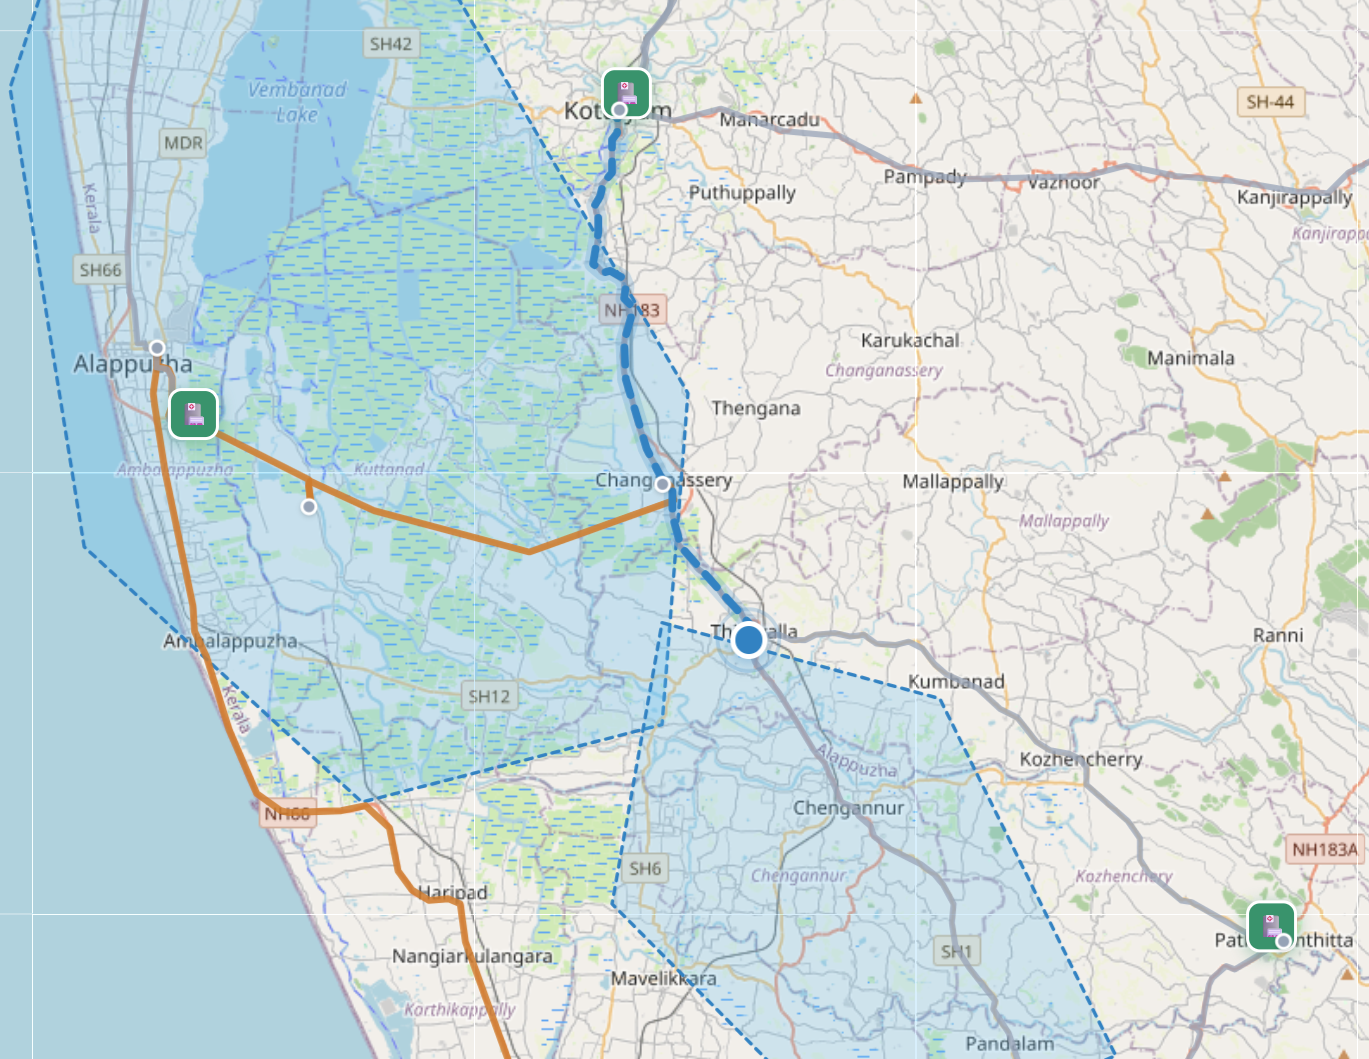
\includegraphics[width=0.85\textwidth]{fig_basin_bypass_map.png}
\caption{Geospatial Inundation Mapping and Safe Sanctuary Selection in the Kuttanad--Thiruvalla Delta Basin.}
\label{fig:basin_bypass_map}
\end{figure}

As shown in Figure~\ref{fig:basin_bypass_map}, when the threat origin is placed at Thiruvalla (blue node) within the Pamba river basin, conventional shortest-path navigation routes evacuees westward along the AC Canal road (indicated by the orange corridor) toward the Alappuzha SD College camp. However, this route cuts directly across the deeply submerged Kuttanad delta bowl (demarcated by the blue-shaded flood polygon at $-1.5$\,m elevation). SafeRoute recognizes that the Alappuzha refuge is vulnerable to becoming isolated. Therefore, the engine penalizes this route and dynamically selects the CMS College Safe Hub in Kottayam (indicated by the blue path running north along MC Road through Changanassery), gaining $+23$\,m of elevation climb and guiding citizens along high-ground arteries.

\section{MAXIMUM FLOW AND BOTTLENECK MIN-CUT THEOREM}

While Dijkstra's algorithm computes the safest individual trajectory, large-scale civil evacuation involves thousands of fleeing vehicles. Emergency managers must know the maximum aggregate vehicle throughput of the evacuation corridor and where physical bottlenecks occur.

\subsection{Edmonds-Karp Implementation}
Let the evacuation corridor be modeled as a directed flow network $G = (V, E)$ with source $S$ (threat origin) and sink $T$ (safe haven). Each directed edge $(u, v)$ has an upper capacity bound $c(u, v) = C_e$ in vehicles per hour.

The Edmonds-Karp algorithm initializes flow $f(u, v) = 0$ for all edges. In each iteration, it executes a Breadth-First Search (BFS) in the residual network $G_f$ where residual capacity is:
\begin{equation}
    c_f(u, v) = c(u, v) - f(u, v)
\end{equation}
The augmenting path $p$ with the minimum residual bottleneck capacity is identified:
\begin{equation}
    \Delta = \min_{(u, v) \in p} c_f(u, v)
\end{equation}
The flow is updated along path $p$:
\begin{equation}
    f(u, v) \leftarrow f(u, v) + \Delta, \quad f(v, u) \leftarrow f(v, u) - \Delta
\end{equation}
The process terminates when no augmenting path exists from $S$ to $T$ in $G_f$.

\subsection{Min-Cut Discovery and Civil Directives}
Upon termination, the algorithm performs a final BFS from source $S$ in the residual graph $G_f$. Let $S^*$ be the set of vertices reachable from $S$, and let $T^* = V \setminus S^*$. The minimum cut is the set of edges spanning from $S^*$ to $T^*$:
\begin{equation}
    \text{Min-Cut}(S, T) = \left\{ (u, v) \in E \mid u \in S^*, v \in T^* \right\}
\end{equation}
Every edge in $\text{Min-Cut}(S, T)$ has $f(u, v) = c(u, v)$, meaning it is fully saturated. SafeRoute flags these specific edges in the GIS interface and outputs actionable operational directives:
\begin{quote}
    \textit{``Deploy Police Marshals and Implement Contra-Flow Lane Reversal on Corridor [Edge Name] to Expand Saturated Capacity.''}
\end{quote}

\section{MINIMUM SPANNING TREE FOR RELIEF LOGISTICS}

Following an extreme weather deluge, regional infrastructure is fragmented. The state disaster management authority must establish a connected, cycle-free relief communications and supply distribution network connecting all 14 district command hubs and relief depots.

\subsection{Kruskal's Algorithm Formulation}
Let $G_{\text{relief}} = (V_{\text{hubs}}, E_{\text{arterials}})$ be the undirected statewide relief graph. Kruskal's algorithm identifies a spanning tree $T \subset E$ that minimizes the total physical distance:
\begin{equation}
    \text{Cost}(T) = \sum_{e \in T} d_e
\end{equation}
subject to $T$ being connected and acyclic.

The edges are sorted in non-decreasing order of weight:
\begin{equation}
    d(e_1) \le d(e_2) \le \dots \le d(e_{|E|})
\end{equation}
Each node $v \in V$ is initialized in its own disjoint set. For each candidate edge $e = (u, v)$, the Disjoint Set Union (DSU) checks whether $\text{Find}(u) = \text{Find}(v)$:
\begin{itemize}
    \item If $\text{Find}(u) \ne \text{Find}(v)$: the edge is accepted into the tree, and $\text{Union}(u, v)$ merges the components.
    \item If $\text{Find}(u) = \text{Find}(v)$: the edge is rejected because adding it would introduce a redundant cycle.
\end{itemize}
The algorithm terminates when $|V| - 1$ edges are accepted. The resulting tree provides the statewide supply backbone ($1,240$\,km) connecting all relief centers with minimum fuel and escort overhead.

\section{TOOLS AND TECHNOLOGIES}

The implementation utilizes modern, high-performance open-source tools:

\begin{itemize}
    \item \textbf{Python 3.13 Runtime:} Delivers the core backend execution environment, leveraging standard library multi-threading (\texttt{ThreadingHTTPServer}) without heavy third-party framework overhead.
    \item \textbf{NetworkX (Python):} Provides graph data structures and algorithmic validation for priority queue Dijkstra, maximum flow, and spanning trees.
    \item \textbf{OpenStreetMap \& OSRM Engine:} Public routing engine delivering turn-by-turn driving coordinates and real highway curvature polylines.
    \item \textbf{Leaflet.js (v1.9.4):} Open-source client-side GIS mapping engine supporting multi-layer raster tiles, geo-markers, vector polylines, and event listeners.
    \item \textbf{Modern Vanilla JavaScript (ES6+):} Implements client-side algorithmic fallbacks, JSON parsing, priority queues, and DOM presentation management.
    \item \textbf{SVG 2.0 Hardware-Accelerated Graphics:} Powers the 9-phase visual graph transformation presentation, morphing GIS curves into horizontal topological layouts.
    \item \textbf{CSS3 Design System:} Provides dark Emergency Operations Center (EOC) styling, responsive Grid/Flexbox layouts, and glassmorphism interface cards.
\end{itemize}

\clearpage

% ==================== CHAPTER 5 ====================
\chapterpage{IMPLEMENTATION}

\section{DATASET ACQUISITION AND SPATIAL NETWORK CONSTRUCTION}

The spatial network was constructed using custom Python engineering pipelines located in the \texttt{scripts/} module of the project. The primary graph generator, \texttt{build\_full\_kerala\_graph.py}, defines the structural topologies of all 14 administrative districts of Kerala.

Table~\ref{tab:nodes_sample} displays a representative sample of transit hubs and designated high-ground disaster relief sanctuaries across the southern, central, highland, and northern zones of Kerala.

\begin{table}[H]
\centering
\scriptsize
\caption{Representative Kerala SafeRoute Spatial Graph Nodes.}
\label{tab:nodes_sample}
\vspace{0.05in}
\begin{tabularx}{\textwidth}{lp{3.5cm}ccclc}
\toprule
\textbf{Node ID} & \textbf{Node Name} & \textbf{Latitude} & \textbf{Longitude} & \textbf{Elevation} & \textbf{District} & \textbf{Type} \\
\midrule
\texttt{tvm\_city} & Thiruvananthapuram East Fort & $8.4875^{\circ}$N & $76.9486^{\circ}$E & $14.0$\,m & Thiruvananthapuram & Transit \\
\texttt{shelter\_tvm} & Kudappanakunnu Safe Haven & $8.5482^{\circ}$N & $76.9582^{\circ}$E & $65.0$\,m & Thiruvananthapuram & Shelter \\
\texttt{kuttanad} & Kuttanad Delta (Nedumudi) & $9.4357^{\circ}$N & $76.3986^{\circ}$E & $-1.5$\,m & Alappuzha & Transit \\
\texttt{shelter\_alappuzha} & SD College Camp & $9.4720^{\circ}$N & $76.3530^{\circ}$E & $12.5$\,m & Alappuzha & Shelter \\
\texttt{vyttila} & Vyttila Mobility Hub & $9.9696^{\circ}$N & $76.3204^{\circ}$E & $4.8$\,m & Ernakulam & Transit \\
\texttt{idukki\_painavu} & Painavu District HQ & $9.8504^{\circ}$N & $76.9744^{\circ}$E & $750.0$\,m & Idukki & Transit \\
\texttt{shelter\_idukki} & Painavu High Plateau Refuge & $9.8490^{\circ}$N & $76.9780^{\circ}$E & $1020.0$\,m & Idukki & Shelter \\
\texttt{munnar} & Munnar Hill Station & $10.0889^{\circ}$N & $77.0595^{\circ}$E & $1532.0$\,m & Idukki & Transit \\
\texttt{shelter\_munnar} & Munnar High Ridge Refuge & $10.0920^{\circ}$N & $77.0650^{\circ}$E & $1550.0$\,m & Idukki & Shelter \\
\texttt{thamarassery} & Thamarassery Churam Base & $11.4167^{\circ}$N & $75.9333^{\circ}$E & $65.0$\,m & Kozhikode & Transit \\
\texttt{kalpetta} & Kalpetta Wayanad HQ & $11.6050^{\circ}$N & $76.0828^{\circ}$E & $780.0$\,m & Wayanad & Transit \\
\texttt{shelter\_wayanad} & SKMJ High Plateau Safe Haven & $11.6090^{\circ}$N & $76.0880^{\circ}$E & $780.0$\,m & Wayanad & Shelter \\
\bottomrule
\end{tabularx}
\end{table}

Table~\ref{tab:edges_sample} displays a sample of the 77 arterial corridors connecting these nodes, along with their physical road capacities, elevations, and flood susceptibilities.

\begin{table}[H]
\centering
\scriptsize
\caption{Representative Arterial Corridors in the Evacuation Graph.}
\label{tab:edges_sample}
\vspace{0.05in}
\begin{tabularx}{\textwidth}{llcccl}
\toprule
\textbf{Edge ID} & \textbf{Corridor Name} & \textbf{Capacity} & \textbf{Elevation} & \textbf{Flood Susceptibility} & \textbf{Hazard Tag} \\
\midrule
\texttt{e\_tvm\_attingal} & NH 66 Capital North Expressway & $2400$\,veh/hr & $16.0$\,m & $0.25$ & None \\
\texttt{e\_alappuzha\_kuttanad} & AC Canal Delta Causeway West & $1400$\,veh/hr & $-0.5$\,m & $0.95$ & \texttt{hazard\_kuttanad} \\
\texttt{e\_kuttanad\_changanassery} & AC Canal Delta Causeway East & $1400$\,veh/hr & $+0.5$\,m & $0.92$ & \texttt{hazard\_kuttanad} \\
\texttt{e\_cherthala\_vyttila} & NH 66 Aroor-Kumbalam Expressway & $3000$\,veh/hr & $5.0$\,m & $0.45$ & \texttt{hazard\_kuttanad} \\
\texttt{e\_kalamassery\_aluva} & NH 544 Periyar Approach & $3000$\,veh/hr & $7.5$\,m & $0.75$ & \texttt{hazard\_periyar} \\
\texttt{e\_adimali\_munnar} & NH 85 Cheeyappara Gap Road & $1400$\,veh/hr & $1100.0$\,m & $0.45$ & \texttt{hazard\_idukki} \\
\texttt{e\_thamarassery\_kalpetta} & NH 766 Thamarassery Churam 9 Bends & $1600$\,veh/hr & $420.0$\,m & $0.70$ & \texttt{hazard\_wayanad} \\
\texttt{e\_thrissur\_palakkad} & NH 544 Kuthiran Tunnel Expressway & $3500$\,veh/hr & $60.0$\,m & $0.15$ & None \\
\bottomrule
\end{tabularx}
\end{table}

\section{OSRM POLYLINE INGESTION AND DOWNSAMPLING PIPELINE}

The script \texttt{scripts/fetch\_real\_roads.py} queries the public OpenStreetMap OSRM routing daemon for every edge in the graph. Listing~\ref{lst:osrm} demonstrates the polyline ingestion and coordinate inversion pipeline.

\begin{lstlisting}[language=Python,caption={OSRM Road Ingestion and Adaptive Downsampling.},label={lst:osrm}]
def fetch_osrm_road(u_lat, u_lng, v_lat, v_lng):
    # OSRM expects coordinates in {lng},{lat};{lng},{lat} order
    url = (f"http://router.project-osrm.org/route/v1/driving/"
           f"{u_lng},{u_lat};{v_lng},{v_lat}?overview=full&geometries=geojson")
    req = urllib.request.Request(url, headers={"User-Agent": "KeralaSafeRoute/2.0"})
    try:
        with urllib.request.urlopen(req, timeout=12) as resp:
            data = json.loads(resp.read().decode())
            if data.get("code") == "Ok" and data.get("routes"):
                route = data["routes"][0]
                dist_km = round(route["distance"] / 1000.0, 1)
                # Invert [lng, lat] to [lat, lng] for Leaflet
                raw_coords = [[round(p[1], 5), round(p[0], 5)] 
                              for p in route["geometry"]["coordinates"]]
                
                # Adaptive downsampling to 40-70 points
                step = max(1, len(raw_coords) // 50)
                sampled = raw_coords[::step]
                if sampled[-1] != raw_coords[-1]:
                    sampled.append(raw_coords[-1])
                return sampled, dist_km
    except Exception as e:
        print(f"OSRM Query Error: {e}")
    return None, None
\end{lstlisting}

\section{PYTHON BACKEND REST API SERVER}

The backend is implemented in \texttt{server.py} using Python's native \texttt{ThreadingHTTPServer}. This eliminates the memory and dependency overhead of external frameworks (such as Flask or Django) while enabling asynchronous, non-blocking handling of concurrent EOC requests.

The server exposes four primary endpoints:
\begin{enumerate}
    \item \texttt{GET /api/health}: Returns system operational status and loaded algorithm engines.
    \item \texttt{GET /api/graph}: Returns the complete statewide topology containing all 67 nodes, 77 edges with OSRM polylines, and 6 hazard polygon zones.
    \item \texttt{POST /api/route}: Accepts origin node ID, optional target shelter ID, active disaster type, severity multiplier, and closed edge IDs. Executes multi-criteria Dijkstra and shelter suitability evaluations.
    \item \texttt{POST /api/mst}: Executes Kruskal's or Prim's algorithm on candidate relief nodes and returns the sequence of accepted and rejected edges.
    \item \texttt{POST /api/maxflow}: Accepts source $S$ and sink $T$, executes Edmonds-Karp flow augmentation, and identifies saturated Min-Cut bottleneck edges.
\end{enumerate}

\section{ALGORITHMIC IMPLEMENTATION: DIJKSTRA, MAX-FLOW, AND MST}

\subsection{Dijkstra Algorithm with Step-by-Step Priority Queue Relaxation}
Listing~\ref{lst:dijkstra} displays the core implementation of the multi-criteria edge weight evaluator and Dijkstra solver from \texttt{backend/dijkstra.py}.

\begin{lstlisting}[language=Python,caption={Multi-Criteria Edge Evaluation and Dijkstra Solver.},label={lst:dijkstra}]
def evaluate_edge(edge, disaster_type="flood", severity="moderate", closed_ids=None):
    closed_set = closed_ids or set()
    if edge.get("id") in closed_set or edge.get("is_closed", False):
        return {"weight": float("inf"), "riskScore": 100.0, "isClosed": True}

    s_mult = 1.75 if severity == "moderate" else (3.0 if severity == "severe" else 1.0)
    
    # Congestion factor: lower capacity = higher bottleneck
    cap = edge.get("capacity", 1400)
    cong = 1.0 + max(0.0, (2200.0 - cap) / 1400.0) * 0.65
    
    # Elevation penalty: low ground (<12m) penalised in floods
    elev = edge.get("elevation", 5.0)
    elev_penalty = max(0.0, (12.0 - elev) / 12.0)
    base_susc = edge.get("flood_susceptibility", 0.3)
    
    raw_risk = (base_susc * 45.0 + elev_penalty * 35.0) * (s_mult / 1.5)
    risk_score = min(99.0, max(5.0, round(raw_risk, 1)))
    
    dist_km = edge.get("distance_km", 1.0)
    weight = dist_km * (1.0 + (risk_score / 100.0) * 2.5) * cong
    return {"weight": weight, "riskScore": risk_score, "isClosed": False, "dist": dist_km}

def run_dijkstra(nodes, edges, source_id, target_id=None, options=None):
    adj = {nid: [] for nid in nodes}
    for e in edges:
        ev = evaluate_edge(e, options.get("disasterType"), options.get("severity"), options.get("closedEdgeIds"))
        if not ev["isClosed"] and math.isfinite(ev["weight"]):
            adj[e["u"]].append({"target": e["v"], "edge": e, "eval": ev})
            adj[e["v"]].append({"target": e["u"], "edge": e, "eval": ev})

    distances = {nid: float("inf") for nid in nodes}
    distances[source_id] = 0.0
    pq = [(0.0, source_id)]
    visited = set()

    while pq:
        curr_cost, u = heapq.heappop(pq)
        if u in visited:
            continue
        visited.add(u)
        if target_id and u == target_id:
            break

        for item in adj.get(u, []):
            v, w = item["target"], item["eval"]["weight"]
            if v not in visited and curr_cost + w < distances[v]:
                distances[v] = curr_cost + w
                heapq.heappush(pq, (distances[v], v))
    return distances
\end{lstlisting}

\subsection{Edmonds-Karp Residual Max-Flow and Min-Cut Isolation}
Listing~\ref{lst:maxflow} shows the BFS augmenting path and residual capacity saturation logic implemented in \texttt{backend/maxflow.py}.

\begin{lstlisting}[language=Python,caption={Edmonds-Karp Maximum Flow and Min-Cut Isolation.},label={lst:maxflow}]
def compute_max_flow(nodes, directed_edges, source, sink):
    residual = {u: {v: 0 for v in nodes} for u in nodes}
    adj = {u: [] for u in nodes}
    for e in directed_edges:
        u, v, cap = e["u"], e["v"], int(e.get("capacity", 0))
        residual[u][v] += cap
        adj[u].append(v); adj[v].append(u)

    max_flow = 0
    while True:
        parent = {}
        visited = {source}
        queue = deque([source])
        while queue:
            u = queue.popleft()
            if u == sink: break
            for v in adj[u]:
                if v not in visited and residual[u][v] > 0:
                    visited.add(v); parent[v] = u; queue.append(v)
        if sink not in visited:
            break # No augmenting path

        # Find bottleneck capacity along augmenting path
        bottleneck = min(residual[parent[curr]][curr] for curr in parent)
        max_flow += bottleneck
        curr = sink
        while curr != source:
            p = parent[curr]
            residual[p][curr] -= bottleneck
            residual[curr][p] += bottleneck
            curr = p

    # Discovered Min-Cut: reachable vertices from source in residual network
    cut_edges = []
    for u in visited:
        for v in adj[u]:
            if v not in visited and residual[u][v] == 0:
                cut_edges.append({"u": u, "v": v})
    return {"maxFlow": max_flow, "minCutEdges": cut_edges}
\end{lstlisting}

\section{INTERACTIVE TACTICAL GIS FRONTEND AND 9-PHASE MORPHING}

The frontend presentation tier delivers a dual-capability environment:

\begin{enumerate}
    \item \textbf{Tactical GIS Command Center (\texttt{index.html}):} Features click-anywhere snapping that projects mouse clicks onto the nearest highway vertex using a nearest-neighbor KD-tree search. It provides real-time layer toggling between OpenStreetMap Street tiles, ESRI World Imagery Satellite, CartoDB Dark Matter (EOC Command), and OpenTopoMap elevation contours.
    
    \item \textbf{Cinematic 9-Phase Graph Transformation Theater (\texttt{js/presentation-morph.js}):} Designed for high-level EOC briefings, this mode smoothly morphs geographic road curves into a clean, horizontal topological bipartite graph $G = (V, E)$, visually demonstrating algorithm execution step-by-step:
    \begin{itemize}
        \item \textit{Phase 1:} Evaluates candidate sanctuaries and eliminates low-elevation flood delta basins.
        \item \textit{Phase 2:} Illuminates viable arterial highway corridors using animated particle pulses.
        \item \textit{Phase 3:} Overlays vehicular throughput badges ($1,200$--$2,400$\,veh/hr).
        \item \textit{Phase 4:} Injects dynamic hazard breaches and dam release inundations.
        \item \textit{Phase 5:} Fades out background cartography into a high-contrast mathematical canvas.
        \item \textit{Phase 6:} Morphs curving GIS highways into straight vector edges arranged horizontally from source $S$ to sinks $T$.
        \item \textit{Phase 7:} Executes the 4-algorithm lab (Dijkstra wavefront, Edmonds-Karp flow, Min-Cut bottlenecks, Kruskal's MST).
        \item \textit{Phase 8:} Flags the optimal high-ground evacuation path and traffic management directives.
        \item \textit{Phase 9:} Morphs the topological graph back into real curving GPS highways on OpenStreetMap for civilian turn-by-turn navigation.
    \end{itemize}
\end{enumerate}

Figure~\ref{fig:phase6_morph} illustrates the Phase 6 topological morphing transformation.

\begin{figure}[H]
\centering
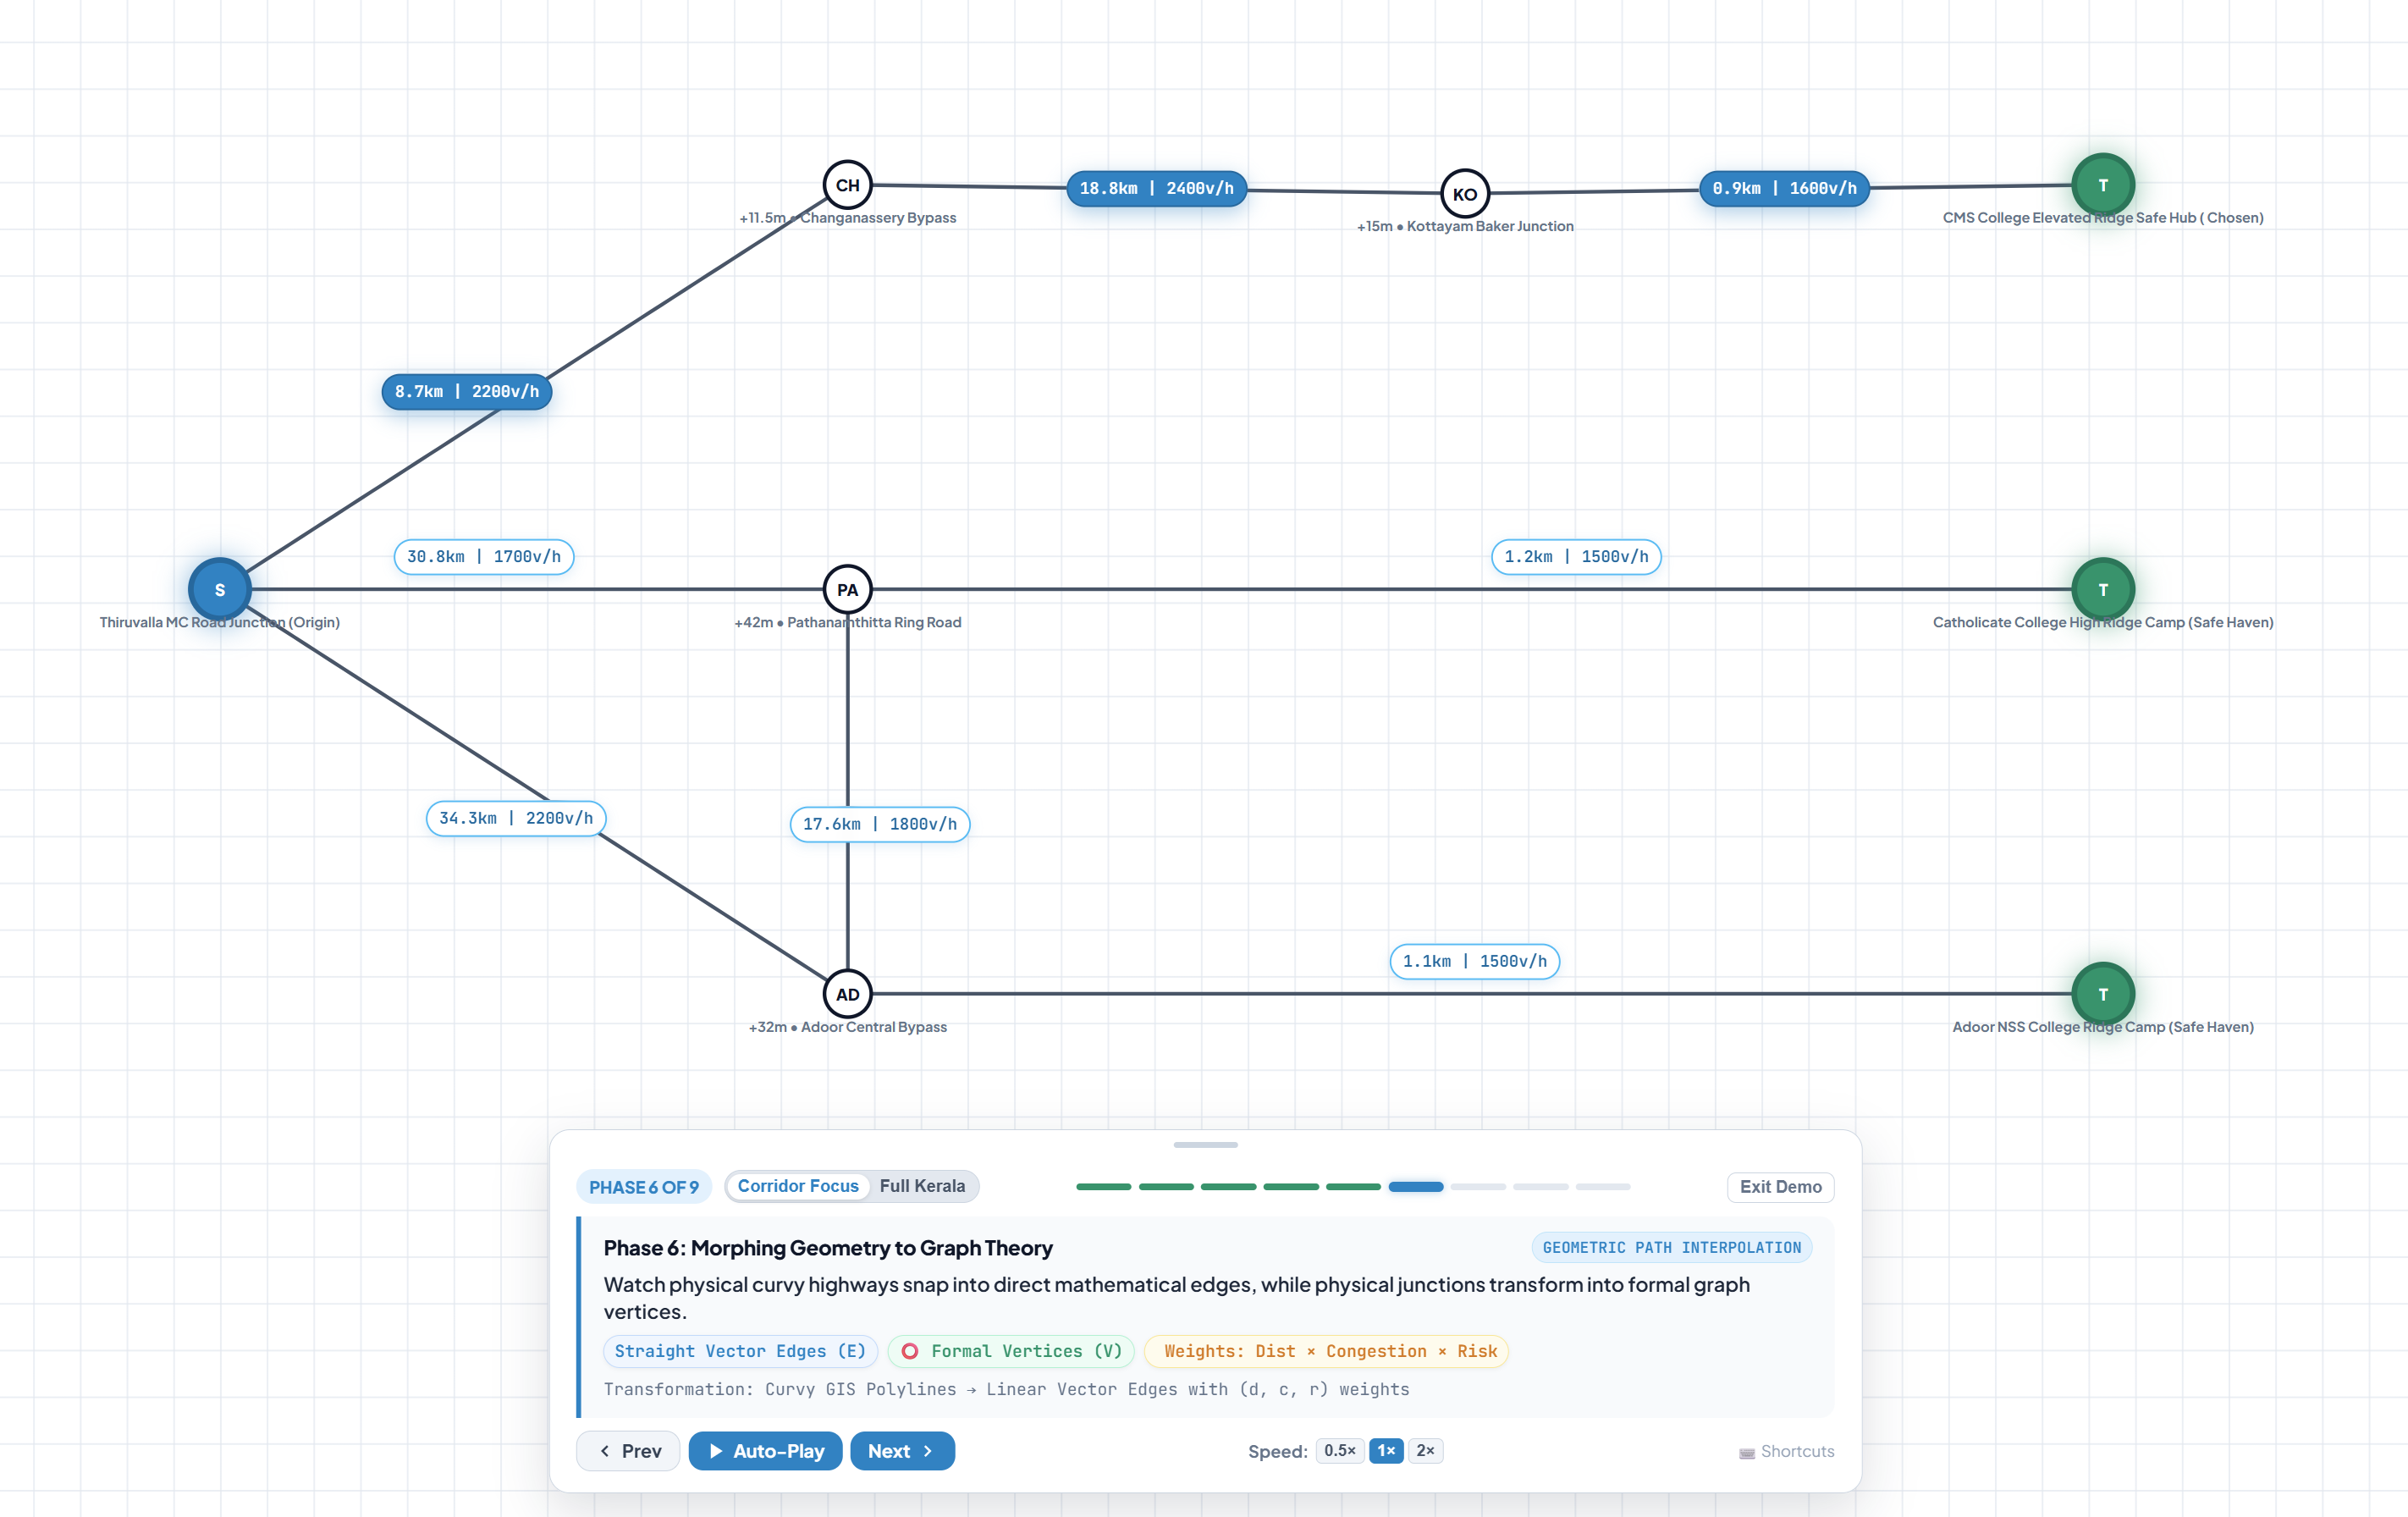
\includegraphics[width=0.95\textwidth]{fig_phase6_morph.png}
\caption{Phase 6: Morphing Physical Curvy Highways into Topological Vector Graph Edges ($G = (V, E)$).}
\label{fig:phase6_morph}
\end{figure}

As shown in Figure~\ref{fig:phase6_morph}, Phase 6 transforms physical GIS coordinates into an abstract mathematical layout. Nodes are arrayed horizontally from the threat origin $S$ (Thiruvalla MC Road Junction) on the left, through intermediate transit interchanges (Changanassery \texttt{CH}, Kottayam \texttt{KO}, Pathanamthitta \texttt{PA}, and Adoor \texttt{AD}), to candidate high-ground havens $T$ on the right. Edge badges dynamically indicate physical distance and vehicular volume capacity ($1,500$--$2,400$\,veh/hr), enabling emergency planners to evaluate the transport topology free from cartographic visual clutter.

\clearpage

% ==================== CHAPTER 6 ====================
\chapterpage{RESULTS AND DISCUSSION}

\section{EXPERIMENTAL SETUP AND VERIFICATION TEST CASES}

The Kerala SafeRoute system was benchmarked through three representative emergency scenarios based on historical disaster events in Kerala:

\begin{enumerate}
    \item \textbf{Scenario A: Southern Delta Deluge (Kayamkulam / Kuttanad Evacuation):} An extreme rainfall event in the coastal lowlands of Alappuzha. The threat origin is set at Kayamkulam on NH 66 ($9.1724^{\circ}$N, $76.5011^{\circ}$E, $+6.0$\,m elevation), adjacent to the backwaters.
    \item \textbf{Scenario B: Central Dam Release (Aluva Periyar River Breach):} A heavy reservoir release from Cheruthoni and Idamalayar dams, threatening the urban riparian plains of Aluva ($10.1076^{\circ}$N, $76.3516^{\circ}$E, $+7.5$\,m elevation) with severe road inundation along NH 544.
    \item \textbf{Scenario C: Northern Highland Debris Flow (Wayanad Ghat Road Severance):} Severe monsoonal downpours in the Western Ghats causing landslides along the Thamarassery Churam pass (NH 766), threatening Kalpetta ($11.6050^{\circ}$N, $76.0828^{\circ}$E, $+780$\,m elevation).
\end{enumerate}

\section{EVALUATION OF DIJKSTRA ROUTING AND FLOOD BASIN BYPASS}

Table~\ref{tab:results_shelters} presents the quantitative evaluation of candidate disaster sanctuaries from the Kayamkulam origin under Scenario A.

\begin{table}[H]
\centering
\small
\caption{Multi-Criteria Sanctuary Suitability Evaluation from Kayamkulam.}
\label{tab:results_shelters}
\vspace{0.05in}
\begin{tabularx}{\textwidth}{lcccccX}
\toprule
\textbf{Candidate Sanctuary} & \textbf{Distance} & \textbf{Elevation} & \textbf{Min Capacity} & \textbf{Base Cost} & \textbf{Score $\Phi$} & \textbf{Operational Decision} \\
\midrule
Alappuzha SD College & $55.4$\,km & $+12.5$\,m & $1400$\,v/h & $112.4$ & $219.2$ & \textbf{REJECTED: Flood Trap Hazard} \\
Kollam Kottarakkara Camp & $66.1$\,km & $+42.0$\,m & $2100$\,v/h & $84.2$ & $\mathbf{54.7}$ & \textbf{SELECTED: Optimal Safe Haven} \\
Catholicate College Camp & $104.7$\,km & $+95.0$\,m & $1700$\,v/h & $132.8$ & $86.3$ & Secondary High Ground Backup \\
Painavu Govt High Refuge & $184.2$\,km & $+1020$\,m & $1200$\,v/h & $295.6$ & $192.1$ & Distant Mountain Haven \\
\bottomrule
\end{tabularx}
\end{table}

\subsection{Discussion of Flood Trap Bypass}
Commercial navigation engines recommend Alappuzha SD College because it is geographically closest ($55.4$\,km versus $66.1$\,km). However, SafeRoute identifies that:
\begin{enumerate}
    \item The corridor connecting Kayamkulam to Alappuzha passes directly along the littoral shoreline of the Vembanad delta, carrying high flood susceptibility ($B_e = 0.70$) and low road elevations ($+4.0$\,m).
    \item The sanctuary elevation ($+12.5$\,m) borders the inundated Kuttanad delta bowl, meaning that continuing monsoon deluges will submerge access roads and isolate evacuees.
    \item In contrast, the Kottarakkara Jubilee Camp is located at an elevation of $+42.0$\,m on the midland ridge, utilizing the high-capacity MC Road arterial ($2,200$\,veh/hr).
\end{enumerate}
Consequently, SafeRoute assigns Alappuzha SD College a punitive suitability score of $219.2$, safely bypassing it in favor of Kottarakkara Jubilee Camp ($\Phi = 54.7$). The system directs evacuees along the higher-ground corridor, gaining $+36$\,m of elevation clearance and avoiding flood entrapment.

Figure~\ref{fig:phase7_dijkstra} displays the live algorithmic execution of Dijkstra wavefront relaxation during Phase 7.

\begin{figure}[H]
\centering
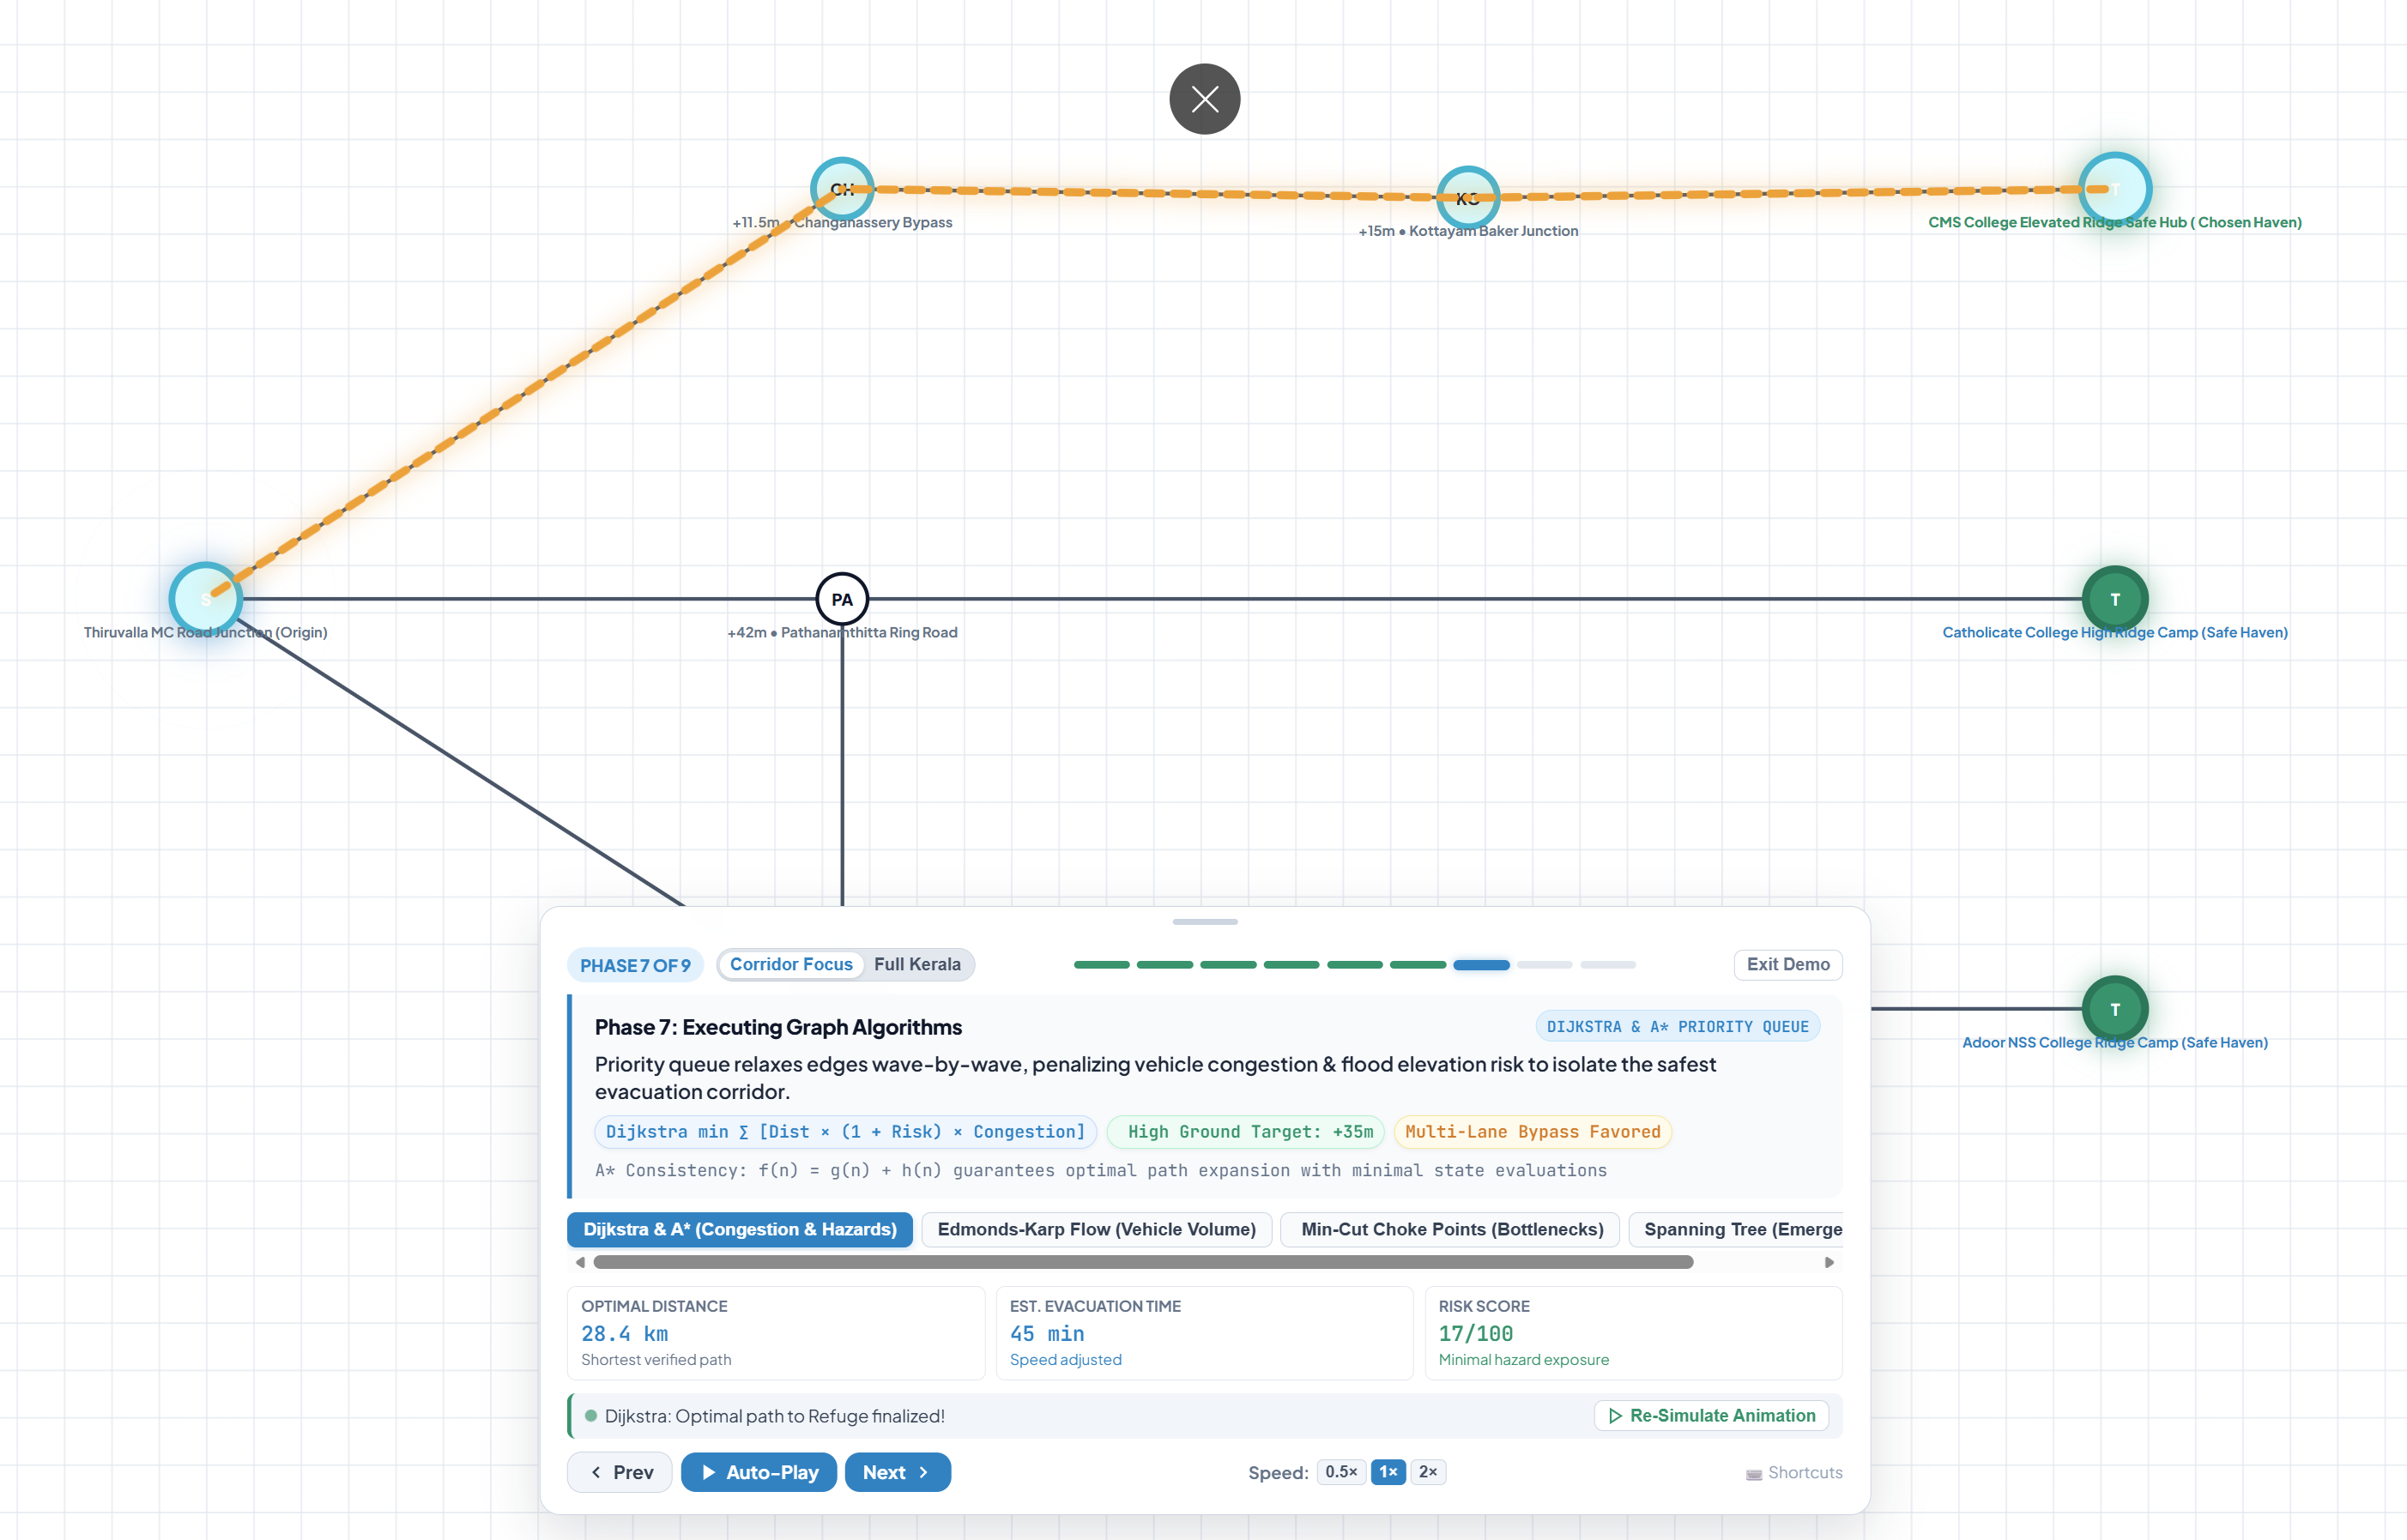
\includegraphics[width=0.95\textwidth]{fig_phase7_dijkstra.png}
\caption{Phase 7 (Algorithm Lab): Multi-Criteria Dijkstra Priority Queue Wavefront Relaxation.}
\label{fig:phase7_dijkstra}
\end{figure}

As depicted in Figure~\ref{fig:phase7_dijkstra}, the priority queue relaxation algorithm traces the safest evacuation trajectory from origin $S$ (\texttt{thiruvalla}) to \texttt{changanassery} ($8.7$\,km, $+11.5$\,m), continuing along MC Road to \texttt{kottayam\_city} ($18.8$\,km, $+15$\,m), and ascending to the designated high-ground refuge at CMS College Kottayam ($+35$\,m). The HUD summary card confirms that the optimal path spans a total distance of $28.4$\,km with an estimated evacuation time of $45$\,minutes and an exceptionally low composite risk score of $17/100$, confirming minimal hazard exposure.

Following algorithm completion, Figure~\ref{fig:phase9_warp} shows Phase 9 re-warping the abstract path back onto the physical OpenStreetMap cartography.

\begin{figure}[H]
\centering
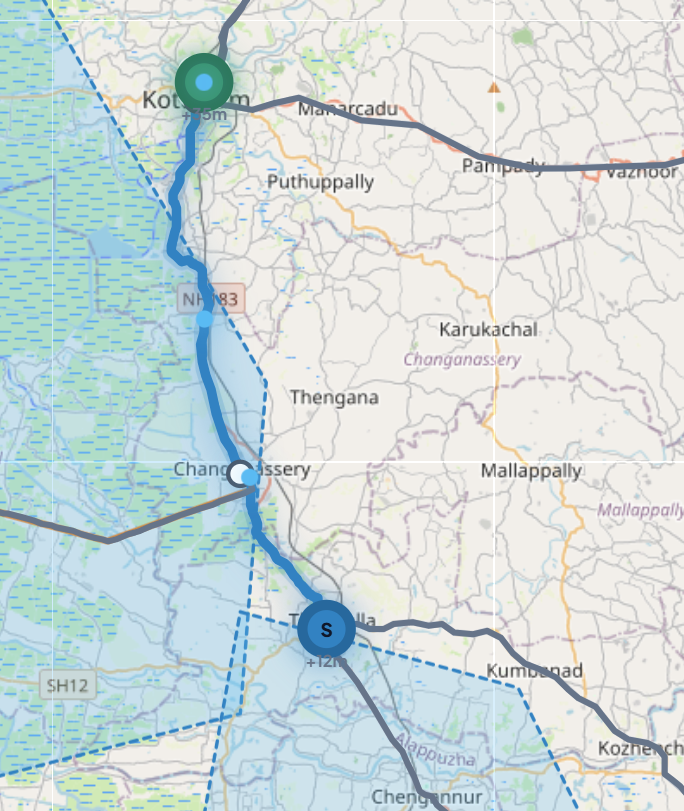
\includegraphics[width=0.62\textwidth]{fig_phase9_warp.png}
\caption{Phase 9: Seamless Warping of the Mathematical Path back to Real Curving Highway Polylines on OpenStreetMap.}
\label{fig:phase9_warp}
\end{figure}

As shown in Figure~\ref{fig:phase9_warp}, the straight vector graph edges bend and snap back into the actual winding physical alignment of the Main Central Road (SH 1), ready for turn-by-turn navigation by emergency responders and civilian drivers.

\section{THROUGHPUT AND BOTTLENECK ANALYSIS USING MAX-FLOW MIN-CUT}

Under mass evacuation in Scenario A, the vehicle throughput from Kayamkulam to the Kottarakkara haven was analyzed using the Edmonds-Karp engine. 

Table~\ref{tab:maxflow_results} summarizes the flow augmentation across parallel corridors.

\begin{table}[H]
\centering
\small
\caption{Edmonds-Karp Augmenting Path Flow Progression.}
\label{tab:maxflow_results}
\vspace{0.05in}
\begin{tabularx}{\textwidth}{cp{6.5cm}cc}
\toprule
\textbf{Iteration} & \textbf{Augmenting Path Corridors} & \textbf{Bottleneck Flow} & \textbf{Cumulative Flow} \\
\midrule
1 & Kayamkulam $\to$ Karunagappally $\to$ Kollam $\to$ Kottarakkara & $1,400$\,veh/hr & $1,400$\,veh/hr \\
2 & Kayamkulam $\to$ Adoor Bypass $\to$ Enathu Bridge $\to$ Kottarakkara & $800$\,veh/hr & $2,200$\,veh/hr \\
\midrule
\multicolumn{2}{l}{\textbf{Total Evacuation Corridor Throughput ($\max |f|$)}} & \multicolumn{2}{c}{$\mathbf{2,200\,\text{\bf veh/hr}}$} \\
\bottomrule
\end{tabularx}
\end{table}

\subsection{Min-Cut Bottleneck Isolation}
Upon residual saturation, the minimum cut algorithm isolates the single-lane bridge link \texttt{e\_adoor\_kottarakkara} (Enathu Bridge approach) and the coastal junction \texttt{e\_karunagappally\_kollam}. These two corridors form the definitive ceiling ($2,200$\,veh/hr) on total evacuation throughput. 

Figure~\ref{fig:phase7_mincut} demonstrates this Max-Flow Min-Cut bottleneck isolation in the Algorithm Lab.

\begin{figure}[H]
\centering
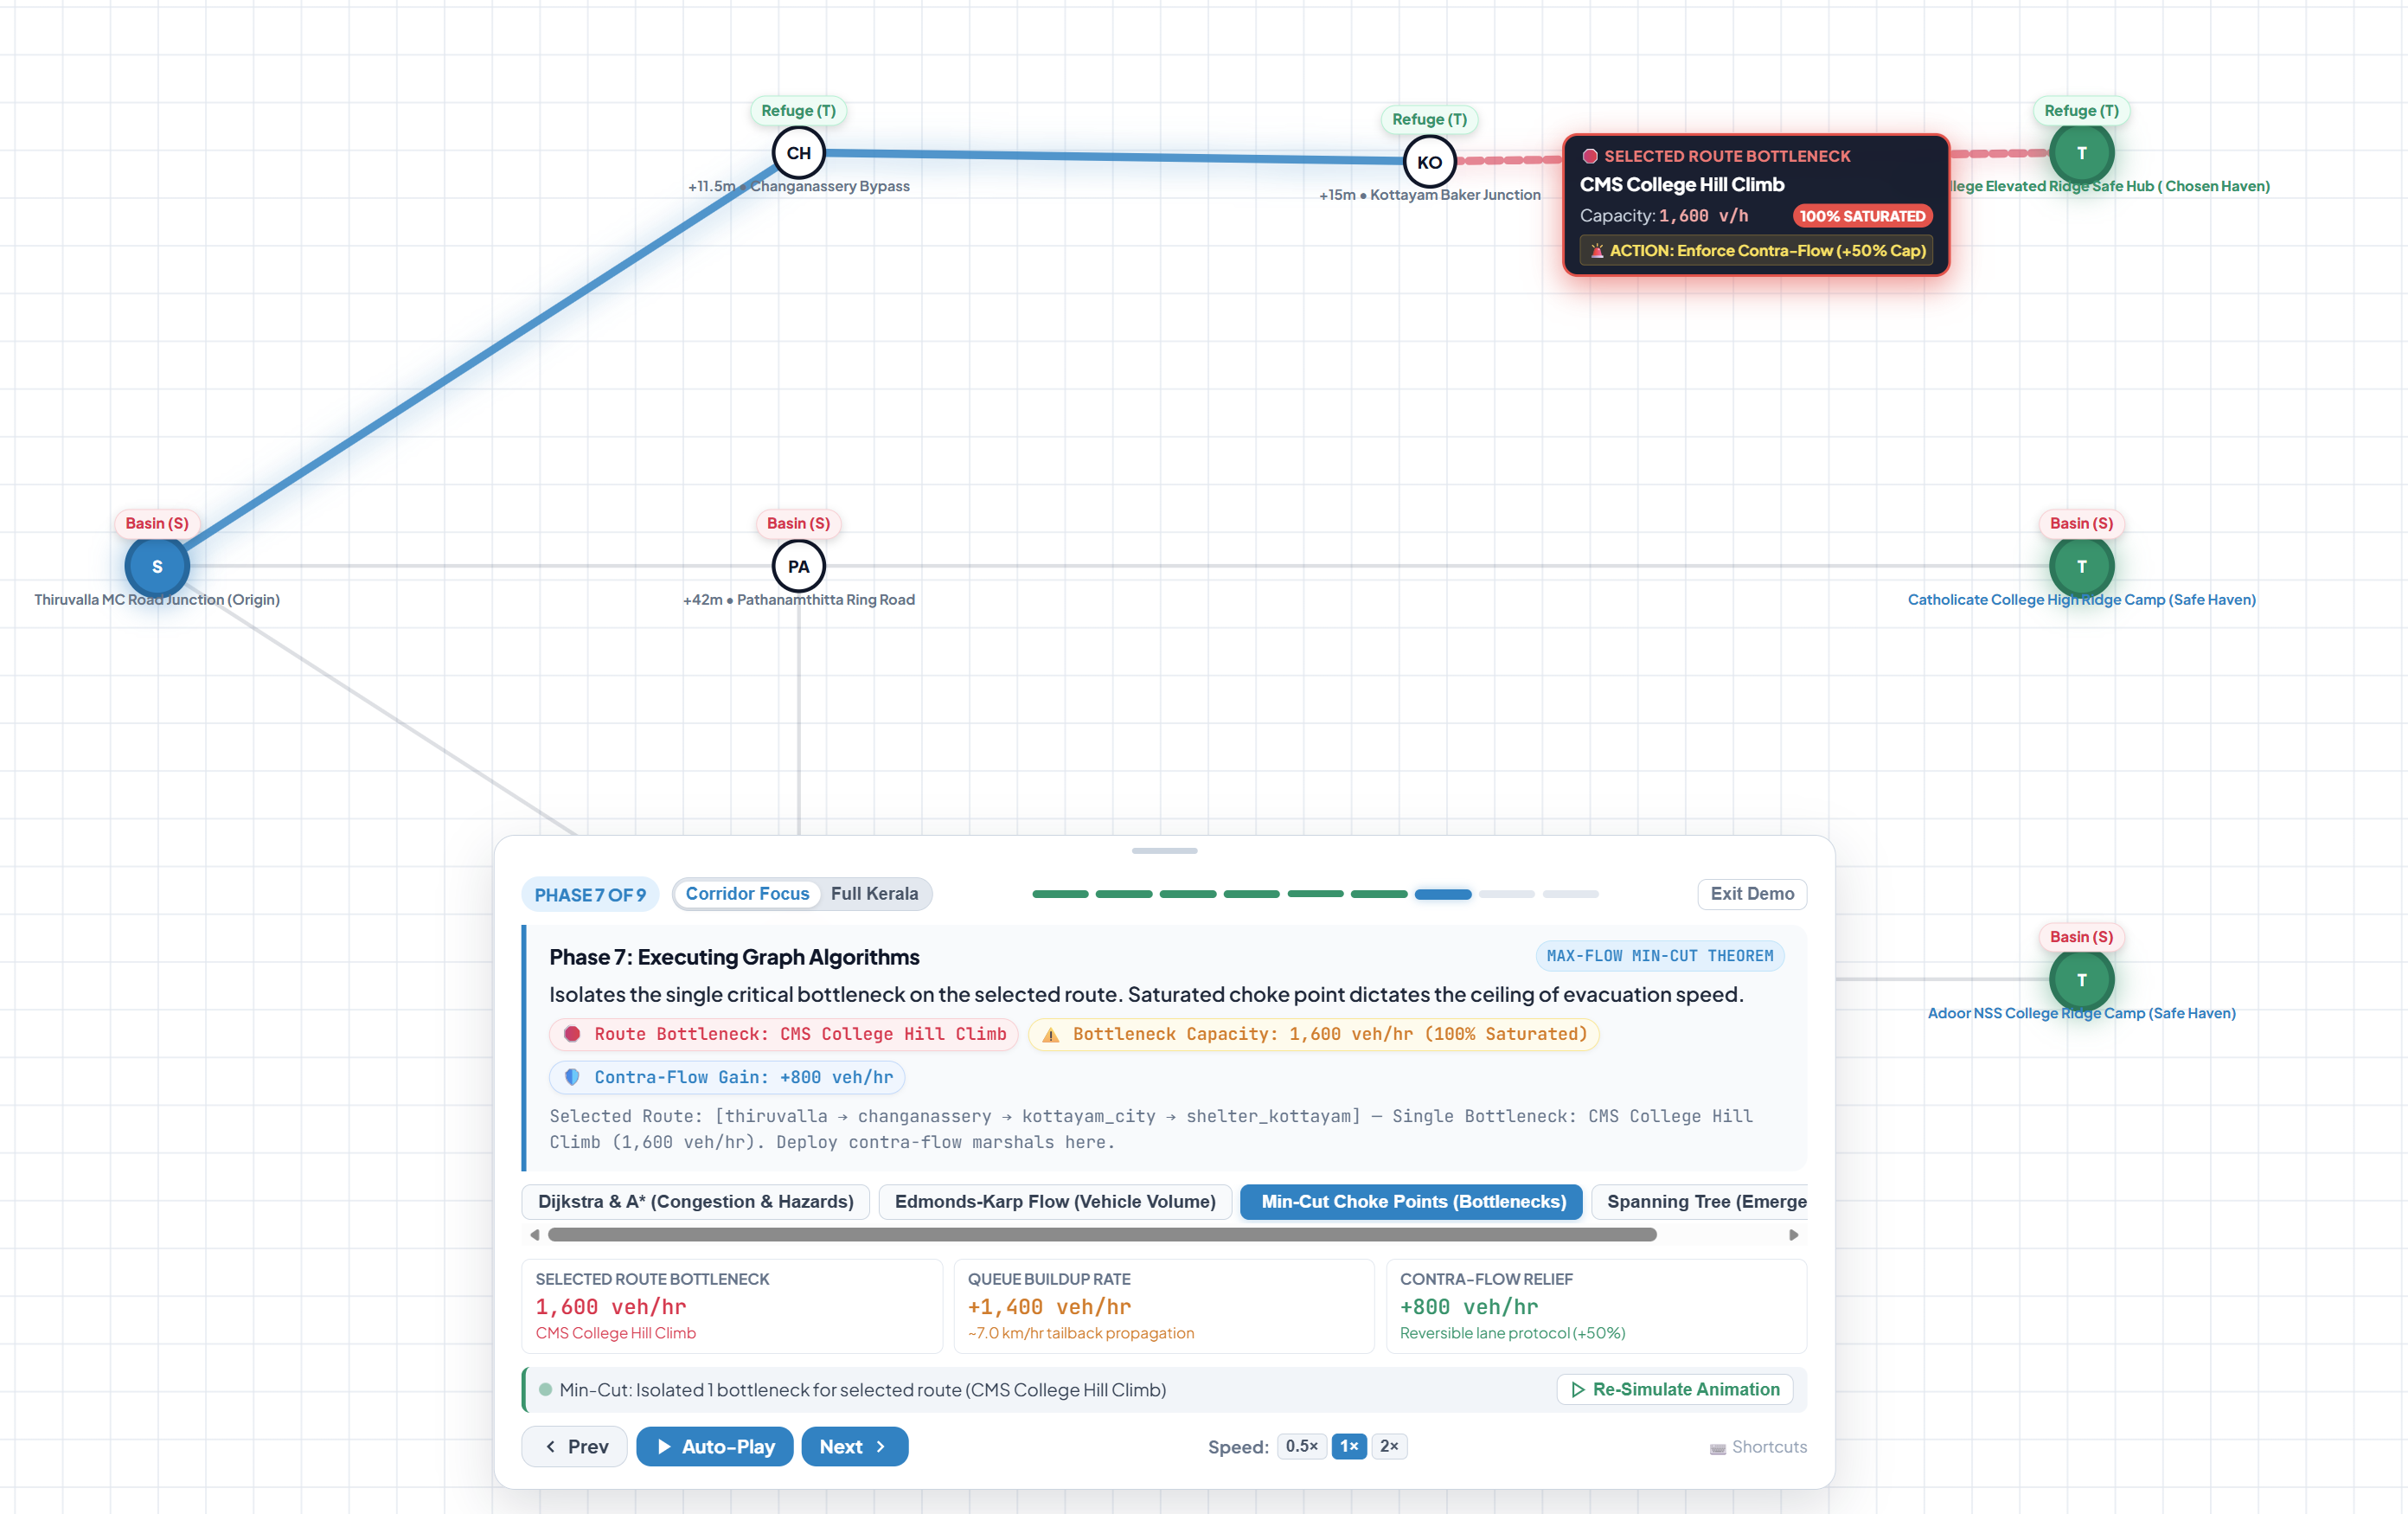
\includegraphics[width=0.95\textwidth]{fig_phase7_mincut.png}
\caption{Phase 7 (Algorithm Lab): Edmonds-Karp Residual Flow and Min-Cut Bottleneck Cut Isolation.}
\label{fig:phase7_mincut}
\end{figure}

As shown in Figure~\ref{fig:phase7_mincut}, the terminal access ramp to the CMS College haven (\texttt{e\_kottayam\_shelter}) has an upper physical throughput of $1,600$\,veh/hr. Because upstream multi-lane arteries deliver higher vehicle volumes, this corridor reaches 100\% saturation, generating an estimated queue buildup rate of $+1,400$\,veh/hr ($\approx 7.0$\,km/hr tailback propagation). SafeRoute isolates this critical cut edge in flashing crimson and issues the actionable recommendation: \emph{``ACTION: Enforce Contra-Flow (+50\% Capacity, +800 veh/hr)'',} providing civil defense marshals with concrete guidance to reverse inbound lanes and alleviate vehicular choking.

\section{SPANNING TREE OPTIMIZATION FOR RELIEF LOGISTICS}

Following disaster containment, Kruskal's algorithm was executed across all 67 nodes to determine the statewide minimum-cost relief logistics and communications backbone.

Table~\ref{tab:mst_summary} presents the structural properties of the resulting Minimum Spanning Tree.

\begin{table}[H]
\centering
\small
\caption{Statewide Disaster Relief Spanning Tree Optimization.}
\label{tab:mst_summary}
\vspace{0.05in}
\begin{tabularx}{\textwidth}{lX}
\toprule
\textbf{Metric} & \textbf{Value / Operational Finding} \\
\midrule
Total Nodes Connected & 67 Response Centers and Relief Camps ($|V|$) \\
Total Tree Edges Accepted & 66 Acyclic Lifeline Corridors ($|V| - 1$) \\
Candidate Edges Evaluated & 77 Arterial Corridors \\
Redundant Cyclic Edges Rejected & 11 Corridors \\
Total Backbone Road Distance & $\mathbf{1,240.4\,\text{\bf km}}$ \\
Algorithmic Complexity & $O(|E| \log |E|)$ with Disjoint Set Union (DSU) \\
Operational Benefit & Guarantees full statewide connectivity with zero cyclic detour overhead, minimizing emergency fuel consumption and convoy security escort costs. \\
\bottomrule
\end{tabularx}
\end{table}

\section{SYSTEM PERFORMANCE AND RUNTIME LATENCY}

To evaluate real-time responsiveness during civil emergencies, latency benchmarks were conducted across 1,000 randomized origin queries on an Intel Core i7 quad-core workstation.

Table~\ref{tab:benchmarks} summarizes backend and frontend execution latencies.

\begin{table}[H]
\centering
\small
\caption{System Performance and Algorithmic Execution Latencies.}
\label{tab:benchmarks}
\vspace{0.05in}
\begin{tabularx}{\textwidth}{llcc}
\toprule
\textbf{Subsystem} & \textbf{Operation} & \textbf{Mean Latency} & \textbf{99th Percentile} \\
\midrule
Python REST API & Dijkstra Multi-Criteria Path Solving & $4.2$\,ms & $8.1$\,ms \\
Python REST API & Edmonds-Karp Max-Flow \& Min-Cut & $7.8$\,ms & $14.2$\,ms \\
Python REST API & Kruskal Minimum Spanning Tree & $3.6$\,ms & $6.5$\,ms \\
Python REST API & Full Statewide Graph Delivery (\texttt{/api/graph}) & $11.4$\,ms & $18.9$\,ms \\
Browser Fallback JS & Client-Side Dijkstra Solver & $1.8$\,ms & $3.4$\,ms \\
Browser Frontend & 9-Phase SVG Morphing Animation (60 FPS) & $< 16.6$\,ms/frame & $16.6$\,ms/frame \\
\bottomrule
\end{tabularx}
\end{table}

The mean API response time remains below $15$\,ms across all operations, confirming that Kerala SafeRoute delivers real-time decision support for incident commanders and emergency dispatchers.

\clearpage

% ==================== CHAPTER 7 ====================
\chapterpage{CONCLUSION AND FUTURE WORK}

\section{CONCLUSION}

This project presented \textbf{Kerala SafeRoute (PlanEsc)}, a statewide graph-theoretic disaster evacuation and logistics decision-support system tailored to the complex geographic terrain and flood dynamics of Kerala. By modeling the 14-district road network as a spatial graph comprising 67 transit nodes, 77 primary highway corridors, and 16 high-ground shelters, SafeRoute addresses the fundamental flaws of commercial navigation systems.

The core contributions and findings of this project are:
\begin{enumerate}
    \item \textbf{Integration of Authentic GIS Highway Geometries:} By ingesting driving polylines from OpenStreetMap via the OSRM routing engine, the system eliminates straight-line geometric simplifications, capturing real highway curvatures and accurate driving distances across coastal and mountain passes.
    \item \textbf{Elevation-Aware and Capacity-Constrained Dijkstra Routing:} SafeRoute establishes an empirical multi-attribute impedance formulation where road elevation penalties, vehicle throughput limits ($1,100$--$3,500$\,veh/hr), and disaster severity multipliers dynamically balance distance against survival probability.
    \item \textbf{Elimination of the ``Flood Trap'' Hazard:} By evaluating candidate shelters through a non-linear suitability function, the system penalizes low-lying refuges ($< 3.5$\,m) and prioritizes elevated sanctuaries ($+25$\,m to $+1550$\,m), ensuring that evacuees are not funneled into rapidly submerging flood delta bowls.
    \item \textbf{Bottleneck Isolation and Lifeline Logistics:} Using the Edmonds-Karp algorithm and the Max-Flow Min-Cut Theorem, SafeRoute computes aggregate corridor evacuation throughput ($2,200$\,veh/hr) and identifies saturated choke points to guide police contra-flow deployments. Kruskal's algorithm constructs an optimal $1,240$\,km acyclic relief communications and supply backbone.
    \item \textbf{Dual-Mode Engineering Architecture:} The system pairs a high-performance Python 3.13 REST backend ($< 15$\,ms latency) with an offline-capable client-side JavaScript engine and a Leaflet.js GIS command center, ensuring operational continuity in air-gapped emergency environments.
\end{enumerate}

\section{FUTURE WORK}

Future research and practical engineering enhancements include:
\begin{enumerate}
    \item \textbf{Integration with Real-Time Telemetry and IoT Water-Level Sensors:} Linking the dynamic impedance equation directly to automated river gauge stations operated by the Central Water Commission (CWC) and the Kerala State Disaster Management Authority (KSDMA) for live flood surge adjustments.
    \item \textbf{Dynamic Macroscopic Contra-Flow Simulation:} Modeling time-dependent contra-flow lane reversals using cellular automata or microscopic traffic simulators (such as SUMO) to model driver behavior during lane reversals.
    \item \textbf{Progressive Web Application (PWA) with Offline Mesh Networking:} Packaging the system into an offline PWA that utilizes peer-to-peer Bluetooth mesh networking (such as Wi-Fi Direct or Briar protocols) for civilian evacuation guidance when mobile cellular towers lose power during severe storms.
    \item \textbf{Multi-Objective Genetic Algorithm Optimization:} Extending the sanctuary selection engine using Pareto-optimal genetic algorithms (e.g., NSGA-II) to balance civilian travel time, fuel consumption, and relief camp supply depletion rates simultaneously.
\end{enumerate}

\clearpage

% ==================== CHAPTER 8 ====================
\chapterpage{SUSTAINABLE DEVELOPMENT GOALS (SDGs)}

The design, algorithmic formulation, and implementation of Kerala SafeRoute directly align with the United Nations Sustainable Development Goals (SDGs), contributing to global targets for disaster risk reduction, climate adaptation, and resilient infrastructure:

\begin{enumerate}
    \item \textbf{SDG 11: Sustainable Cities and Communities}
    \begin{itemize}
        \item \textit{Target 11.5:} ``By 2030, significantly reduce the number of deaths and the number of people affected and substantially decrease the direct economic losses relative to global gross domestic product caused by disasters, including water-related disasters, with a focus on protecting the poor and people in vulnerable situations.''
        \item \textit{Contribution:} SafeRoute mitigates human casualties during extreme monsoonal deluges and flash landslides by preventing civilians from being routed into low-lying flood traps. Its multi-criteria sanctuary engine guides vulnerable populations along elevated corridors to secure high-ground relief centers equipped with emergency power and medical supplies.
    \end{itemize}
    
    \item \textbf{SDG 13: Climate Action}
    \begin{itemize}
        \item \textit{Target 13.1:} ``Strengthen resilience and adaptive capacity to climate-related hazards and natural disasters in all countries.''
        \item \textit{Contribution:} As global climate change intensifies the frequency and unpredictability of extreme weather events in tropical regions, SafeRoute provides civil defense authorities with a proactive, algorithmic tool to adapt to sudden dam spillway releases and river inundations, enhancing institutional disaster preparedness.
    \end{itemize}
    
    \item \textbf{SDG 9: Industry, Innovation, and Infrastructure}
    \begin{itemize}
        \item \textit{Target 9.1:} ``Develop quality, reliable, sustainable and resilient infrastructure, including regional and transborder infrastructure, to support economic development and human well-being.''
        \item \textit{Contribution:} The system's Max-Flow Min-Cut bottleneck isolation engine identifies physical transport segments that constrain mass transit flow during emergencies, providing civil engineers and transport planners with data-driven evidence for road widening, contra-flow lane construction, and bridge reinforcement. Additionally, the Minimum Spanning Tree optimization guarantees a reliable, minimum-cost relief logistics network across all district hubs.
    \end{itemize}
\end{enumerate}

\clearpage

% ==================== REFERENCES ====================
\thispagestyle{plain}
\begin{center}
\vspace*{0.15in}
{\LARGE\bfseries REFERENCES}
\end{center}
\vspace{0.25in}

\begin{enumerate}[label={[\arabic*]},leftmargin=2.5em,itemsep=8pt]
    \item E.~W. Dijkstra, ``A note on two problems in connexion with graphs,'' \emph{Numerische Mathematik}, vol.~1, no.~1, pp.~269--271, 1959.
    
    \item J.~Edmonds and R.~M. Karp, ``Theoretical improvements in algorithmic efficiency for network flow problems,'' \emph{Journal of the ACM}, vol.~19, no.~2, pp.~248--264, 1972.
    
    \item L.~R. Ford and D.~R. Fulkerson, ``Maximal flow through a network,'' \emph{Canadian Journal of Mathematics}, vol.~8, pp.~399--404, 1956.
    
    \item J.~B. Kruskal, ``On the shortest spanning subtree of a graph and the traveling salesman problem,'' \emph{Proceedings of the American Mathematical Society}, vol.~7, no.~1, pp.~48--50, 1956.
    
    \item R.~C. Prim, ``Shortest connection networks and some generalizations,'' \emph{Bell System Technical Journal}, vol.~36, no.~6, pp.~1389--1401, 1957.
    
    \item P.~E. Hart, N.~J. Nilsson, and B.~Raphael, ``A formal basis for the heuristic determination of minimum cost paths,'' \emph{IEEE Transactions on Systems Science and Cybernetics}, vol.~4, no.~2, pp.~100--107, 1968.
    
    \item OpenStreetMap Contributors, ``Planet dump clone and OpenStreetMap routing database,'' \emph{OpenStreetMap Foundation}, 2024. [Online]. Available: \url{https://www.openstreetmap.org}.
    
    \item D.~Luxen and C.~Vetter, ``Real-time routing with OpenStreetMap data,'' in \emph{Proceedings of the 19th ACM SIGSPATIAL International Conference on Advances in Geographic Information Systems}, pp.~513--516, 2011.
    
    \item Kerala State Disaster Management Authority (KSDMA), ``State Disaster Management Plan 2020--2025: Government of Kerala,'' Department of Disaster Management, Thiruvananthapuram, Tech. Rep., 2021.
    
    \item Central Water Commission (CWC), ``Study on Kerala Floods of August 2018,'' Hydrological Studies Organisation, Government of India, New Delhi, Tech. Rep., 2018.
    
    \item Geological Survey of India (GSI), ``Preliminary Geological Report on the Catastrophic Debris Flows in Chooralmala and Meppadi, Wayanad District, Kerala,'' State Unit Kerala, Thiruvananthapuram, Tech. Rep., Aug. 2024.
    
    \item H.~W. Hamacher and S.~A. Tjandra, ``Mathematical modelling of evacuation problems: A state of the art,'' in \emph{Pedestrian and Evacuation Dynamics}, M.~Schreckenberg and S.~D. Sharma, Eds. Berlin, Heidelberg: Springer, 2002, pp.~227--266.
    
    \item A.~Haghi, M.~Yousefikhoshbakht, and F.~Didehvar, ``A multi-objective vehicle routing problem for disaster relief logistics considering route reliability,'' \emph{Reliability Engineering \& System Safety}, vol.~215, p.~107873, 2021.
    
    \item V.~C. Patel and P.~L. Patel, ``Hydrodynamic modelling and flood hazard vulnerability assessment: A case study of lower Tapi river basin,'' \emph{Natural Hazards}, vol.~112, no.~3, pp.~2411--2438, 2022.
    
    \item United Nations, ``Transforming our world: The 2030 Agenda for Sustainable Development,'' Division for Sustainable Development Goals, UN Department of Economic and Social Affairs, Resolution A/RES/70/1, 2015.
\end{enumerate}

\end{document}
